%        File: Stanford_Machine_Learning_Notes.tex
%     Created: Mon May 18 11:00 pm 2020 E
% Last Change: Mon May 18 11:00 pm 2020 E
%
\documentclass[letter]{article}
\title{%
    Machine Learning\\
    \large Stanford University \\
    Professor Andrew Ng}

\author{Jordan Hong}
\newcommand*{\vertbar}{\rule[-1ex]{0.5pt}{2.5ex}} % for complicated matrices
\newcommand*{\horzbar}{\rule[.5ex]{2.5ex}{0.5pt}}
\date{\today}
\usepackage{graphicx}
\usepackage{amsfonts}
\usepackage{caption}
\usepackage{subcaption}
%\usepackage{color}   %May be necessary if you want to color links
\usepackage{hyperref}
\hypersetup{
    linktoc=all     %set to all if you want both sections and subsections linked
}
\usepackage{amsmath}
\usepackage{listings}
\usepackage{color} %red, green, blue, yellow, cyan, magenta, black, white
\usepackage[T1]{fontenc}
% macro to select a scaled-down version of Bera Mono (for instance)
\makeatletter
\newcommand\BeraMonottfamily{%
  \def\fvm@Scale{0.85}% scales the font down
  \fontfamily{fvm}\selectfont% selects the Bera Mono font
}
\makeatother

\definecolor{mygreen}{RGB}{28,172,0} % color values Red, Green, Blue
\definecolor{mylilas}{RGB}{170,55,241}
\lstset{language=Matlab,%
    basicstyle=\BeraMonottfamily,
    breaklines=true,%
    frame=single,%
    morekeywords={matlab2tikz},%
    keywordstyle=\color{blue},%
    morekeywords=[2]{1}, keywordstyle=[2]{\color{black}},%
    identifierstyle=\color{black},%
    stringstyle=\color{mylilas},%
    commentstyle=\color{mygreen},%
    showstringspaces=false,%without this there will be a symbol in the places where there is a space
    emph=[1]{for,end,break},emphstyle=[1]\color{red}, %some words to emphasise
    %emph=[2]{word1,word2}, emphstyle=[2]{style},    
    gobble=8,%
    tabsize=4
}
\usepackage{algorithm, algorithmic}
\newlength\myindent % define a new length \myindent
\setlength\myindent{2em} % assign the length 2em to \myindet
\newcommand\bindent{%
  \begingroup % starts a group (to keep changes local)
  \setlength{\itemindent}{\myindent} % set itemindent (algorithmic internally uses a list) to the value of \mylength
  \addtolength{\algorithmicindent}{\myindent} % adds \mylength to the default indentation used by algorithmic
}
\newcommand\eindent{\endgroup} % closes a group


\begin{document}
\maketitle
\tableofcontents
\newpage
    \section{Introduction}
    \subsection{What is Machine Learning}
    
    \begin{enumerate}
        \item Machine Learning 
            \begin{itemize}
                \item Grew out of work in Artificial Intelligence (AI)
                \item New capabilities for computers
            \end{itemize}
        \item Examples: 
            \begin{itemize}
                \item database mining
                \item applications can't programby hand (handwriting recognition, Natural Language Processing (NLP), Computer Vision) 
                \item Neuromorphic applications
            \end{itemize}
           
        \item Definition
            \begin{itemize}
                \item Arthur Samuel(1959) \\
                    \begin{quote}
                        Machine Learning: Field of study that gives computers the ability to learn without being explicitly programmed.

                    \end{quote}
                \item Tom Mitchell(1998) \\
                    \begin{quote}
                         Well-posed Learning Problem: A computer program is said to learn from experience E with respect to some task T and some performance measure P, if its performance on T, as measured by P, improves with experience E. 

                    \end{quote}
           \end{itemize}
        \item Machine Learning in this course:
            \begin{enumerate}
                \item Suupervised Learning
                \item Unsupervised Learning
                \item Others: reinforcement learning, recommender systems
                \item Practical application techniques
            \end{enumerate}
    \end{enumerate}

    
    \subsection{Supervised Learning}

        In supervised learning, the \emph{the right answer} is given. For example:
        \begin{enumerate}
            \item Regression: predict real-valued output.
            \item Classification: predict discrete-valued output.
        \end{enumerate}

    \begin{figure}[h]
        \centering
        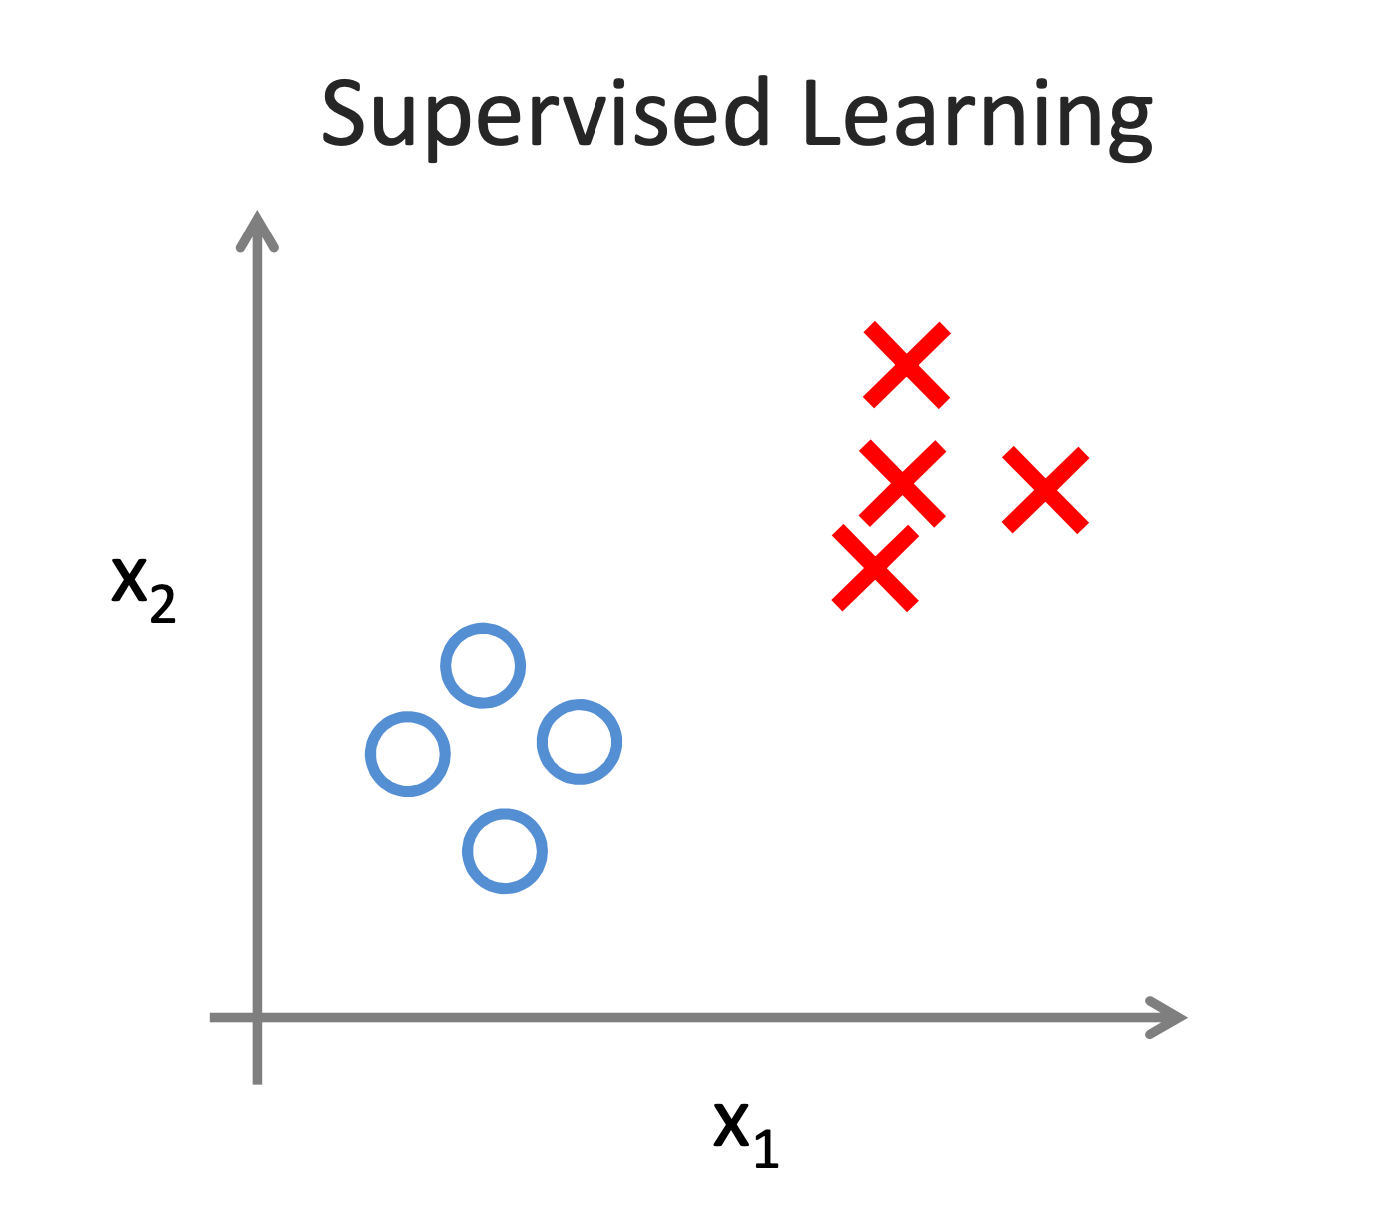
\includegraphics[width=0.5\textwidth]{image/supervised-learning.png}
        \caption{Supervised Learning}
        \label{fig:supervised-learning}
    \end{figure}

    \subsection{Unsupervised Learning}
    The right answer is not given, e.g. cocktail problem (distinguishing two voices from an audio file.)

    \begin{figure}[h]
        \centering
        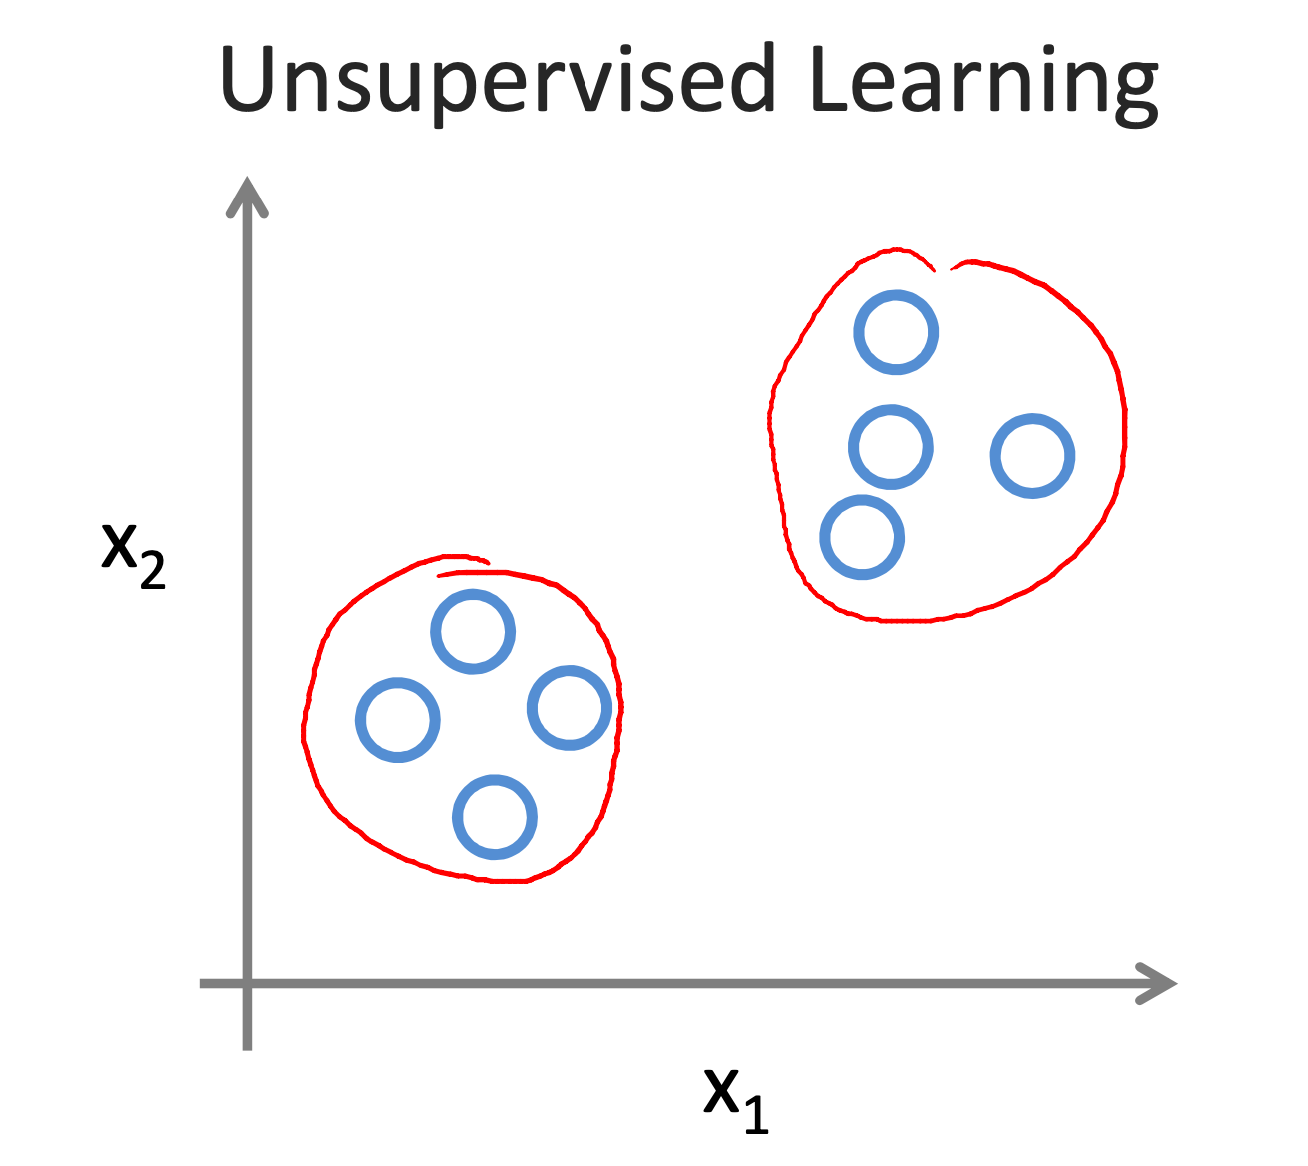
\includegraphics[width=0.5\textwidth]{image/unsupervised-learning.png}
        \caption{Unsupervised learning}
        \label{fig:unsupervised-learning}
    \end{figure}


    \section{Linear Regression with One Variable}
    \subsection{Model Representation}
        \subsubsection{Notations}
            For a training set:
           \begin{itemize}
               \item \textbf{m} = Number of training examples.
               \item \textbf{x} = ``input'' variable / features.
               \item \textbf{y} = ``output'' variables / ``target'' variable.
               \item \textbf{(x,y)} - one training example.
               \item \textbf{(x\textsuperscript{i},y\textsuperscript{i})} denotes the i\textsuperscript{th} training example 

           \end{itemize}

        \subsubsection{Hypothesis Function}
        
           A hypothesis function (h) maps input (x) to estimated output (y).
           How do we represent h?

           \begin{equation} 
               \boxed{ 
                   \textbf{Hypothesis Function}\hspace{10pt}  h_\theta (x) = \theta_0 + \theta_1x
           }
              \label{eq:hypothesis}
           \end{equation}

           We can apply \emph{Univariate linear regression} with respect to x. 
    \subsection{Cost Function}

    Recall \ref{eq:hypothesis}. The $\theta_i$s are parameters we have to choose. The intuition is is that we want to choose $\theta_i$ s such that h\textsubscript{$\theta$} is closest to y for our training examples (x,y).
    

      \begin{equation} 
          \boxed{ 
              \textbf{Cost Function}\hspace{10pt} J(\theta_0, \theta_1) = \frac{1}{2m} \sum_{i=1}^{m} (h_\theta(x^{(i)}) - y^{(i)} )^2
      }
          \label{eq:cost}
      \end{equation}
      

      \par \textbf{Summary} 
      \begin{enumerate}
          \item \textbf{Hypothesis  }$h_\theta (x) = \theta_0 + \theta_1x$
          \item \textbf{Parameters } $\theta_0, \theta_1$
          \item \textbf{Cost Function }$J(\theta_0, \theta_1) = \frac{1}{2m} \sum_{i=1}^{m} (h_\theta(x^{(i)}) - y^{(i)} )^2$
          \item \textbf{Goal } $\min_{\theta_0, \theta_1} J(\theta_0, \theta_1)$
    
      \end{enumerate}
        

          
   
    
    \subsection{Gradient Descent}
        \subsubsection{Intuition}
            \begin{enumerate}
                \item We have some function $J(\theta_0, \theta_1)$, we want to $\min_{\theta_0, \theta_1} J (\theta_0, \theta_1)$
                \item Outline: start with some $\theta_0, \theta_1$, keep changing  $\theta_0, \theta_1$ to reduce $J(\theta_0, \theta_1)$ until we end up at a minimum. 
            \end{enumerate}
        \subsubsection{Gradient Descent Algorithm}
            \textbf{Algorithm} \\
                repeat until convergence\{  
                    \[ \theta_j := \theta_j - \alpha \frac{\partial }{\partial \theta_j} J(\theta_0, \theta_1)\mbox{\hspace{10pt} (for j=0 and j=1)} 
                   .\] \}
        \\


           \textbf{Notes}
               \begin{enumerate}
                   \item the := denotes non-blocking assignment, i.e. simultaneously updates $\theta_0 and \theta_1$ 
                   \item We use the derivative to find a local minimum. 
                   \item $\alpha$ denotes the learning rate. Gradient descent can converge to a local minimum even when the learning rate $\alpha$ is fixed. As we approach a local minimum, gradient descent will automatically take smaller steps. Therefore it is not needed to decrease $\alpha$ over time. 
               \end{enumerate}

       \subsubsection{Gradient Descent with Linear Regression}
     
       Recall, we have:
       \begin{enumerate}
           \item Gradient Descent Algorithm: \\ 
               \linebreak
               repeat until convergence\{  
                    \[ \theta_j := \theta_j - \alpha \frac{\partial }{\partial \theta_j} J(\theta_0, \theta_1)\mbox{\hspace{10pt} (for j=0 and j=1)} 
                   .\] \}


           \item Linear Regression Model:
               \begin{center}
                   \[h_\theta (x) = \theta_0 + \theta_1x\]
                   \[J(\theta_0, \theta_1) = \frac{1}{2m} \sum_{i=1}^{m} (h_\theta(x^{(i)}) - y^{(i)} )^2\]             

               \end{center}

       \end{enumerate}
            
                 
                
    We can substitute the above equations, which gives us:
       \begin{center}
           \[\theta_0 := \theta_0 - \alpha \frac{1}{m} \sum_{i=1}^{m} (h_\theta(x^{(i)}) - y^{(i)} )\] 
               \[\theta_1 := \theta_1 - \alpha \frac{1}{m} \sum_{i=1}^{m} (h_\theta(x^{(i)}) - y^{(i)} ) \cdot x^{(i)}\]  

       
       \end{center} 
    


    \section{Review of Linear Algebra}

This is section is a basic review of linear algebra. I have skipped this section for now and will come back to it if time permits.

    \section{Linear Regression with Multiple Variables}

    \subsection{Multiple features}
    Recall in the single variable case, we have a single input (x), two parameters($\theta_0, \theta_1$). The hypothesis can be expressed as: \[
        h_\theta(x)= \theta_0 + \theta_1x
    .\] 
  
    Now, consider a generalized case where there are multiple features: X\textsubscript{1}, X\textsubscript{2}, X\textsubscript{3}. The information can be organized in a table with example numerical values:
    \begin{table}[htbp]
            \begin{center}
                 \begin{tabular}{||c c c c||} 
                 \hline
                  Sample Number (i) & X\textsubscript{1} &  X\textsubscript{2} & y \\ [0.5eX] 
                 \hline\hline
                 1 & 6 & 87837 & 787 \\ 
                 \hline
                 2 & 7 & 78 & 5415 \\
                 \hline
                 3 & 545 & 778 & 7507 \\
                 \hline
                 4 & 545 & 18744 & 7560 \\
                 \hline
                 5 & 88 & 788 & 6344 \\ [1ex] 
                 \hline
                \end{tabular}
             \caption{Sample Table}
             \label{tab:data}
         \end{center}
     \end{table}


        From Table \ref{tab:data}, one can see that each row is a sample a feature on each column.

    \subsubsection{Notation}

        \begin{enumerate}
            \item \textbf{n}: number of features.
            \item \textbf{x\textsuperscript{(i)}}: (row vector) input features of the i\textsuperscript{th} training example. i= 1, 2,\dots, m. 
            \item \textbf{x\textsuperscript{(i)}\textsubscript{j}}: value of feature j in the i\textsuperscript{th} training example. j= 1, 2, \dots, n.  

        \end{enumerate}

    \subsubsection{Hypothesis}

        Previously, 
        \[ 
        h_\theta(x)= \theta_0 + \theta_1\cdot x 
        \]
    

        Now, we can extend the hypothesis to :

        \[
            h_\theta(x) = \theta_0\cdot1 + \theta_1\cdot x_1 + \theta_2\cdot x_2  
        \]

        For convenience of notation, let's define x\textsubscript{0}=1, i.e. x\textsuperscript{i}\textsubscript{0}=1 $\forall$ i.

        Therefore, we have: \textbf{x}= $\left[ \begin{array}{c}
                                                    x_0 \\
                                                    x_1 \\
                                                    x_2 \\
                                                    \vdots \\
                                                    x_n
                                                 \end{array}
                                          \right]$
                                          and \textbf{$\theta$} = $\left[ \begin{array}{c}
                                                    \theta_0 \\
                                                    \theta_1 \\
                                                    \theta_2 \\
                                                    \vdots \\
                                                    \theta_n \\
                                                 \end{array}
                                          \right]$. 
        Then, the hypothesis function can be written as:

            \begin{equation}
                \begin{split}
                 h_\theta (x) &= \left[ \begin{array}{ccccc}
                                                \theta_0 & \theta_1 & \theta_2 & \dots & \theta_n 
        \end{array} 
                                    \right] \cdot \left[ \begin{array}{c}
                                                                x_0 \\
                                                                x_1 \\
                                                                x_2 \\
                                                                \vdots \\
                                                                x_n
                                                                 \end{array} \right] \\
                                                                 & = \theta^T\cdot \textbf{x}
            \end{split}
        \end{equation}
        

        This is \emph{Multivariate linear regression}.










    \subsection{Gradient Descent for Multiple Variables}
        \subsubsection{Algorithm}
            \textbf{Summary for Multivariables} 
                \begin{enumerate}
                    \item \textbf{Hypothesis  }$h_\theta (x) = \theta^T \cdot \textbf{x}$
                    \item \textbf{Parameters } $\mathbf{\theta}$
                    \item \textbf{Cost Function } $ J(\mathbf{\theta}) = \frac{1}{2m} \sum_{i=1}^{m} (h_\theta(x^{(i)}) - y^{(i)} )^2 $
                    \item \textbf{Goal } $ \min_{\mathbf{\theta}} J( \mathbf{\theta}) $
                \end{enumerate}

        
                \textbf{Gradient Descent for Multiple Variables}
                        repeat until convergence\{  
                            \[ \theta_j := \theta_j - \alpha \frac{\partial }{\partial \theta_j} J(\mathbf{\theta})\mbox{\hspace{10pt} (for j=0, 1,$\ldots$ n)}  
                            \] 
                        \}  \\


                        
                       \[\theta_j := \theta_j - \alpha \frac{1}{m} \sum_{i=1}^{m} (h_\theta(\mathbf{x^{(i)}}) - y^{(i)} ) \cdot x_j^{(i)}\] \\ 
                       
                       Note: $x_0^{(i)} = 1$, by definition.
        
         \subsubsection{Vectorized Implementation}

         One can work out the linear algebra and arrive at the following simplification using vectorized operations.
            The cost function $J$ can be expressed as:
            \begin{equation}
                J(\theta) = \frac{1}{2m} (\mathbf{X\theta} - \mathbf{y})^T (\mathbf{X\theta} - \mathbf{y} )
                \label{eq:vectorized-cost}
            \end{equation}
            
            The MATLAB implementation is as follows:
            \begin{lstlisting}
                m = length(y); % calculate how many samples 
                J = 1/(2*m)*((X*theta-y).')*(X*theta-y);

            \end{lstlisting}


            Gradient descent can be vectorized in the form:
            \begin{equation}
                \theta = \theta - \frac{\alpha}{m} \cdot \mathbf{X}^T \cdot (\mathbf{X\theta} - \mathbf{y}) 
                \label{eq:vectorized-gradient-descent}
            \end{equation}

            The MATLAB implementation is as follows:
            \begin{lstlisting}
                m = length(y); % number of training examples
                for iter = 1:num_iters
                    theta = theta - alpha/m* X.'*(X*theta -y);
            \end{lstlisting}


    \subsection{Gradient Descent in Practise I: Feature Scaling} 
    
        \begin{itemize}
            \item Idea: ensure each featurre are on a similar scale
            \item Get every feature into approx. $-1\leq x_i \leq1 $($\sim$ order)
            \item \textbf{Mean Normalization}: Replace $x_i$ with $\frac{x_i - \mu_i}{s_i}$, where $\mu_i$ and $s_i$ are the sample mean and standard deviation, respectively.

        \end{itemize}

    \subsection{Gradient Descent in Practise II: Learning Rate}
        
        \begin{itemize}
            \item Ensure gradient descent is working: plot $J_\theta$ over each number of iteration (not over $\theta$ !)
            \item Example automatic convergence test: for sufficiently small $\alpha$ $J_\theta$ should decrease by less than $10^{-3}$ i one iteration.
            \item If $\alpha$ is too small, gradient descent can be slow to converge.
            \item If $\alpha$ is too large, gradient descent may not converge.
            \item To choose $\alpha$, try 0.001, 0.003, 0.01, 0.03, 0.1, 0.3, 1\ldots (by 3x)
        \end{itemize}


    \subsection{Features and Polynomial Regression}
        We can fit into different polynomials by choice, using multivariate regression. Recall
        \[
            h_\theta (x) = \theta_0 + \theta_1x_1 + \theta_2x_2 +\theta_3x_3 
        \]  

        Let x\textsubscript{1} be x\textsuperscript{1}, x\textsubscript{2} be x\textsuperscript{2}, x\textsubscript{3} be x\textsuperscript{3}.
        Note we should still apply feature scaling to x\textsubscript{1}, x\textsubscript{2}, and x\textsubscript{3} individually! 


    \subsection{Normal Equation}

        The normal equation provides a method to solve for $\theta$ analytically. For our data with m samples, n features, recall each sample can be written as: 
       \[ 
        \mathbf{x^{(i)}} =  \begin{bmatrix}
            x_0^{(i)}\\
            x_1^{(i)} \\
            x_2^{(i)} \\
            \vdots \\
            x_j^{(i)}\\
           \vdots \\
           x_n^{(i)}
            \end{bmatrix}
        \]
        We can construct a design matrix:
        \[ \mathbf{X} = \begin{bmatrix}
            \horzbar & (x^{(1)})^T & \horzbar \\
            \horzbar & (x^{(2)})^T & \horzbar \\
            \horzbar & (x^{(3)})^T & \horzbar \\
                     & \vdots      &          \\
            \horzbar & (x_{m}^{T}  & \horzbar \\
         \end{bmatrix}
        \]

         Then $\theta$ can be found by the normal equation: 
                 \begin{equation}
                 \mathbf{\theta} = \mathbf{(X^TX)}^{-1}\mathbf{Ty}
                     \label{eq:normal}
                 \end{equation}

        
        Normal equation is useful as no $\alpha$ is required to and we do not need to iterate. However, we do have to compute $(X^TX)^{-1}$, which can be computationally expensive when n is large. The complexity is O($n^3$) for inverse operations. Gradient Descent is useful when n is large (many features). 

     \subsection{Normal Equation and Non-invertibility}

     What if $(X^TX)^{-1}$ is non-invertible? 

     \begin{itemize}
         \item Redundant features (linearly dependent), i.e. having same information in two different units.
         \item Too many features (i.e. m $\leq$ n). Delete some features or use regularization
     \end{itemize}




    \section{Octave/MATLAB Tutorial}

    \section{Logistic Regression}

    \subsection{Classification}
        
        \begin{itemize}
            \item Binary Classification: y $\in \{0, 1\}$, where 0 denotes the negative class; 1 denotes the positive class.
            \item Multi-class Classification:y $\in \{0, 1, \cdots, n\}$ 
        \end{itemize}

        We will be using binary classification: 
        \begin{itemize}
            \item Linear regression is not suitable for classification: since $h_\theta (x)$ can output out of range, i.e. $<0$ or $>1$. 
            \item We will use \textbf{logistic regression}, which ensures that the output $h_\theta (x)$ is between 0 and 1.
        \end{itemize}

    \subsection{Hypothesis Representation}

        \subsubsection{Logistic function}
            The idea is to have $ 0 \leq h_\theta (x) \leq 1$. Instead of the linear regression hypothesis: $h_\theta (x) = \theta^T x$, we will let:
                \[
                    h_\theta (x) = g (\theta^t x)
                ,\]

                where \[
                    g(z) = \frac{1}{1+e^{-z}}
                \]

                g(z) is known as the \textbf{logistic function}, also known as the Sigmoid function. Figure \ref{fig:sigmoid-function} shows a plot of the logistic function, which ranges from 0 to 1. 


                which yields 
                \begin{equation}
                    h_\theta (x) = \frac{1}{1+e^{-z}}
                    \label{eq:log-reg-hypo}
                \end{equation}


                \begin{figure}[htbp]
                    \centering
                    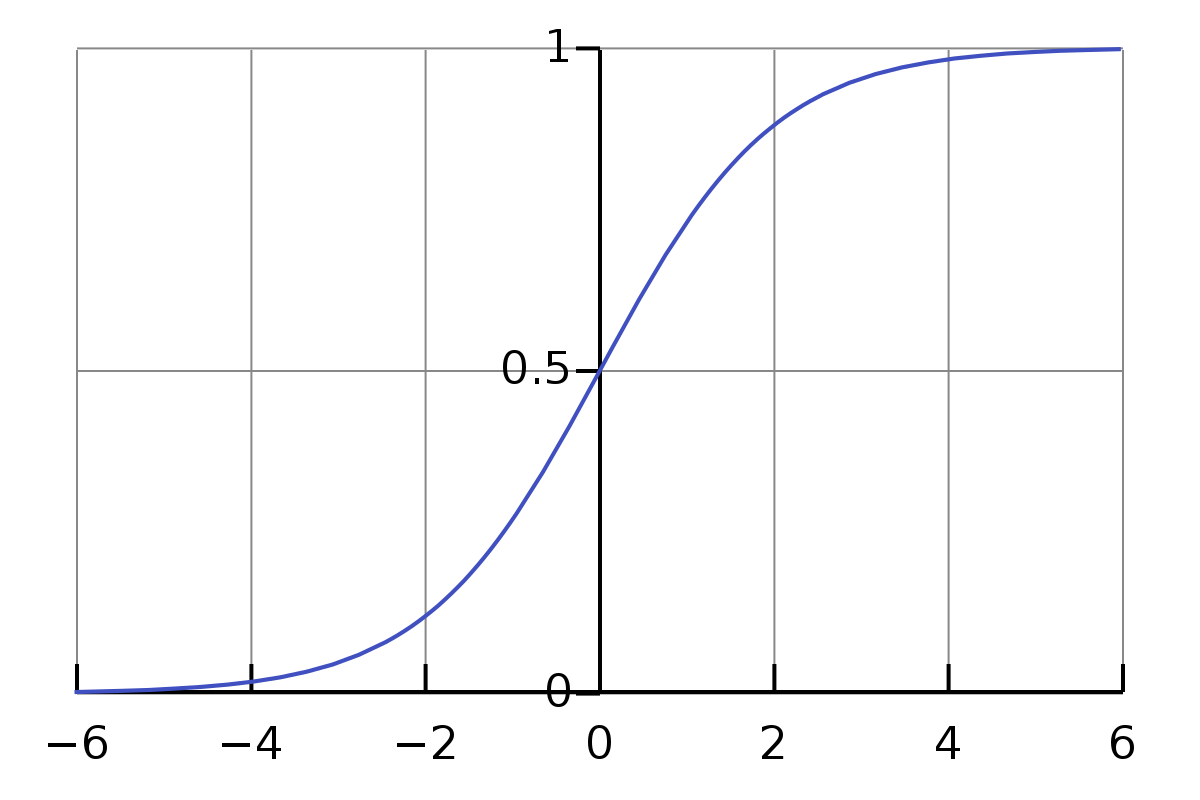
\includegraphics[width=0.5\textwidth]{image/sigmoid-function.png}
                    \caption{Sigmoid Function}
                    \label{fig:sigmoid-function}
                \end{figure}


        \subsubsection{Interpretation of Hypothesis Output}
        $ h_\theta (x)= $ estimated probability that y= 1 on input x. For example, $h_\theta(x)= 0.7$ gives us a probability of 70\% that are output is 1. 
        From a probability theory point of view, one can express $h_\theta (x)$ as $ P(y=1 \mid x;\theta)$. 

        Note that since this is a probability and the total probability sums up to 1, and the real y can only be either 0 or 1:
        \[
            P(y=0 \mid x; \theta) + P(y=1 \mid x;\theta) = 1
        \] 
            


    \subsection{Decision Boundary}

    Recall so far we have $h_\theta (x) = g(\theta^T x)$ and $g(z) = \frac{1}{1+exp(-z)}$. Suppose we set $h_\theta(x) = 0.5$ to be our determining factor for whether y= 0 or y =1. Note that from \ref{fig:sigmoid-function}, one can observe that $h_\theta(x) = 0.5$ corresponds to $\theta^T x = 0$, which is the \textbf{decision boundary}. The decision boundary is the equation which separates the different classes on a plot. There are linear and non-linear decision boundaries.


    \subsection{Cost function}

        Previously, we had $ J(\theta) = \frac{1}{m} \sum_{i=1}^{m} Cost( h_\theta ( x^{(i)}), y^{(i)} )$, where $Cost (h_\theta(x), y) = \frac{1}{2} (h_\theta(x) - y)^2$. 
        Now, the definition of the hypothesis $h_\theta$ has changed to $\frac{1}{1+exp(-\theta^T x}$, as a result the cost function is now non-convex. \\ 
        
            \textbf{Logistic Regression Cost Function}

            Therefore, a new cost function definition is needed. We propose: 

            \[
                Cost (h_\theta(x), y) = 
                \begin{cases}
                    -log(h_\theta(x))       &\quad \text{if } y=1 \\
                    -log(1- h_\theta(x))    &\quad \text{if } y=0 \\
                \end{cases}
            \] 

            Note that Cost=0, if y=1, $h_\theta(x) =1$; but as $h_\theta(x) \to 0$, then $Cost \to \infty$. This proposition captures the intuition that if $h_\theta(x)=0$, predict $P(y=1 \mid x;\theta)$, but y ends up being 1, we will penalize the learning algorithm by very large cost.
            
    \subsection{Simplified Cost Function and Gradient Descent}
        

            Since y can only be either 0 or 1, we can simplify the cost function.
       

            \begin{equation}
                \begin{split}
                    J(\theta)   &= \frac{1}{m}\, \sum_{i=1}^{m}\, Cost\,(\, h_\theta ( x^{(i)})\, ,\, y^{(i)} ) \\
                    &= \frac{-1}{m} \, [ \; \sum_{i=1}^{m}\, y^{(i)}\, log\, h_\theta (x^{(i)})\; +\; (1-y^{(i)})\: log\:(\,1-h_\theta(x^{(i)})\,) \;] 
                \end{split}
                \label{eq:simplified-logistic-cost-function}
            \end{equation}
            Equation \ref{eq:simplified-logistic-cost-function} is based on Maximum Likelihood Estimation.


            A vectorized implementation is, for a design matrix $\mathbf{X}$:
            \begin{equation}
                \boxed{
                    h = g(\mathbf{X\theta})
                }
                \label{eq:vectorized-logistic-hypothesis}
            \end{equation} 

            
            \begin{equation}
                \boxed{
                    J (\theta) = \frac{1}{m} (-y^T log(h) - (1-y)^T log(1-h) )
                }
                \label{eq:vectorized-logistic-cost-function}
            \end{equation} \\

            
            For gradient descent,we would want to $\min_{\theta} J(\theta)$:\\ 

             Repeat \{
                \[ 
                \theta_j := \theta_j - \alpha \frac{\partial }{\partial \theta_j} J(\theta)
                \]

            \} \\

   
            We can compute the partial derivative of $J(\theta)$, which is identical to that of linear regression:
            \[
                \frac{\partial }{\partial \theta_j} J(\theta) = \frac{1}{m} \sum_{i=1}^{m} ( h_\theta (x^{(i)}) - y^{(i)} )\cdot x^{(i)} 
            \]\\
            However, in this case the hypothesis function $h_\theta(x) = \frac{1}{1+exp(-\theta^T x}$ has changed!

            A vectorized implementation for this is:
            \begin{equation}
                \boxed{
                    \mathbf{\theta} := \mathbf{\theta} - \frac{\alpha}{m} \mathbf{X}^T( g (\mathbf{X\theta}) - \mathbf{y}))
                }
                \label{eq:vectorized-logistic-gradient-decent}
            \end{equation}



    \subsection{Advanced Optimization}
        \subsubsection{Taking a Step Back}
            If we take a step back, and consider essentially what tasks we are performing. We need to compute two things:
            \begin{enumerate}
                \item $J(\theta)$
                \item $\frac{\partial}{\partial \theta_j}J(\theta)$
            \end{enumerate}

        \subsubsection{Optimization Algorithm}
        There exists other more sophisticated and faster ways to optimize $\theta$ instead of gradient descent; they often do not involve selecting learning rate $\alpha$ and are more efficient. However, these algorithms are harder to code by hand. It is suggested that we use libraries for such algorithms. 

        We can write a single function that returns both  $J(\theta)$ (jVal) and  $\frac{\partial}{\partial \theta_j}J(\theta)$ (gradient):

        \begin{lstlisting}
        function [jVal, gradient] = costFunction(theta)
            jVal = [...code to compute J(theta)...];
            gradient = [...code to compute derivative of J(theta)...];
        end
            
        \end{lstlisting}

        Then we can use octave's "fminunc()" optimization algorithm along with the "optimset()" function that creates an object containing the options we want to send to "fminunc()".

        \begin{lstlisting}
            options = optimset('GradObj', 'on', 'MaxIter', 100);
            initialTheta = zeros(2,1);
            [optTheta, functionVal, exitFlag] = fminunc(@costFunction, initialTheta, options);
            
        \end{lstlisting}
        

        We then give to the function "fminunc()" our cost function, our initial vector of theta values, and the "options" object that we created beforehand.
        \subsection{Multiclass Classification: One-vs-All}
            Now, let's extend the binary classification of data to multi-classes, i.e expanding our definition of y s.t. y=\{0, 1, \ldots, n\}.
            We will divide out problem into n+1 (0\ldots n) binary classification problems. In each problem, we predict the probability that y is a memember of one of our class. We train a logistic regression classifier $h_\theta ^{(i)} (x) $ $\forall$ i to predict y = i:
            \begin{equation}
                h_\theta^{(i)} (x) = P (y=i \mid x;\theta)
                \label{eq:multiclass-logistic-classifier}
            \end{equation}

            Figure \ref{fig:multi-class-regression} shows an example of the procedure of classifying three classes. We choose one class and then lump all the others into a single second class (hence the name One-vs-All). We apply the binary logisic regression repeatedly and use the hypothesis that returns the highest value. 

            \begin{equation}
                prediction\,=\: \max_{i}\: (\, h_\theta ^{(i)} (x) \,)   
                \label{eq:max-log-regre}
            \end{equation}
            

            \begin{figure}[htbp]
                \centering
                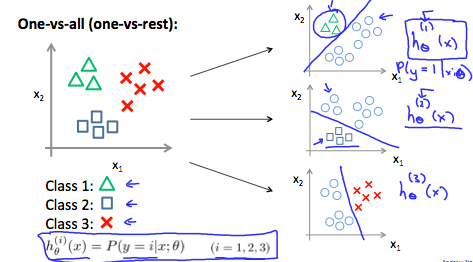
\includegraphics[width=\textwidth]{image/multi-class.png}
                \caption{Example of Multiclass Logistic Regression}
                \label{fig:multi-class-regression}
            \end{figure}

    \section{Regularization}
    \subsection{The problem of overfitting}
    There are two types of errors in fitting functions to data, in which data shows the structure is not captured by the model. The terminology applies to both linear and logistic regression. Figure \ref{fig:fitting} shows an example of each fitting case. 

            \begin{enumerate}
                \item Underfitting (high bias): when the form of our hypothesis function ($h_\theta (x)$) maps poorly to the trend of data. It is usually caused by a function that is either too simple or uses too little features. 
                \item Overfitting (high variance): when hypothesis function learns the training set very well hence fits the available data but does not generalize well to predict new data, i.e fitting too many details. It is usually caused by a complicated function that creates a lot of unneccessary curves and angles unrelated to the data. 
            \end{enumerate}
        
            \begin{figure}[htbp]
                \centering
                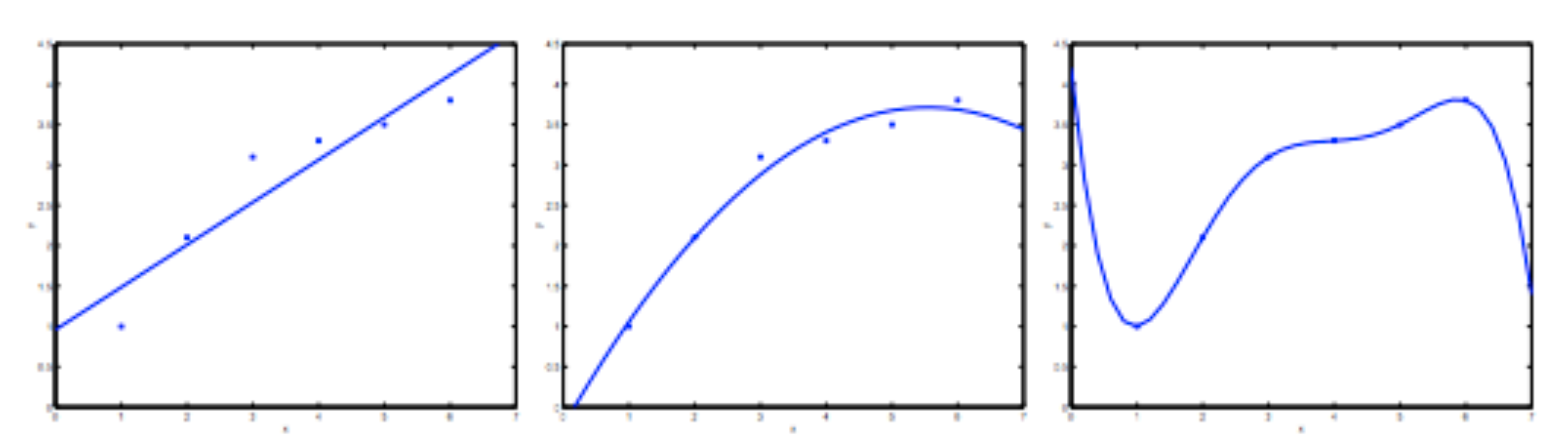
\includegraphics[width=\textwidth]{image/fitting.png}
                \caption{Three scenarios of fitting: underfit(left), good fit (middle), and overfit(right).}
                \label{fig:fitting}
            \end{figure}

        There are two main options to address the issue of overfitting:
            \begin{enumerate}
                \item Reduce the number of features
                    \begin{itemize}
                        \item manually select which features to keep.
                        \item Use a model selection algorithm (later in the course).
                    \end{itemize}
                \item \textbf{Regularization}
                    \begin{itemize}
                        \item Keep all the features, but reduce the magnitude of parameters $\theta_j$
                        \item Regularization worls well when we have a lot of slightly useful features. (Each contributes a bit to predict y)
                    \end{itemize}
            \end{enumerate}


    \subsection{Cost Function}
        \subsubsection{Intuition}
            Suppose we have overfitting, we can reduce the weight that some of the terms in our function carry by penalizing the feature parameter with increased cost. Consider the following hypothesis function : \[
            \theta_0 + \theta_1 x + \theta_2 x^2 + \theta x^3 + \theta x^4
        .\] We would want to make the function more quadratic, which means we would like to reduce the influence of $\theta_3$ and $\theta_4$. Since our goal was to minimize the cost function $J(\theta)$, we could modify the original cost function \[
            \min_\theta \frac{1}{2m} \sum_{i=1}^{m} ( h_\theta (x^{(i)}) - y^{(i)} )^2 + 1000\cdot \theta_3^2 + 1000\cdot \theta_4^2
        .\] This will force $\theta_3$ and $\theta_4$ to be close to zero, and make the original hypothesis function more quadratic.

        \subsubsection{Regularization}
            Now, we can take a step further and regularize all theta parameters: 

            \begin{equation}
                \min_\theta \:\:[ \frac{1}{2m} \sum_{i=1}^{m} ( h_\theta (x^{(i)}) - y^{(i)} )^2 ] + \lambda \sum_{j=1}^{n} \theta_j^2
                \label{eq:regularization-general-form}
            \end{equation}

            Here we are performing two separate operations which can be oberved as the two terms in Equation \ref{eq:regularization-general-form}. The first term corresponds to ``training the data'', and the second term relates to ``keeping the parameters small''. The coefficient $\lambda$ is the \textbf{regularization parameter} and determines the balance between the aforementioned two objectives. Note that if $\lambda$ is too big ($\approx$ 10\textsuperscript{10}), then all $\theta_j \approx 0$, except for $\theta_0$ (the constant term). This makes $h_\theta \approx 0$ and defies the purpose of training and leads to underfitting ( a flat horizontal line).




    \subsection{Regularized Linear Regression}
    \subsubsection{Gradient Descent} 
        We will modify the gradient descent function to separate out $\theta_0$ from the rest of the parameters because we do not want to penalize $\theta_0$.\\

        repeat until convergence\{  
            \[ \theta_0 := \theta_0 - \alpha \frac{1}{m} \sum_{i=1}^{m} ( h_\theta (x^{(i)}) - y^{(i)}) x_0^{(i)}\] 

            \[
                \theta_j := \theta_j - \alpha [ ( \frac{1}{m} \sum_{i=1}^{m} ( h_\theta (x^{(i)}) - y^{(i)}) x_j^{(i)} ) + \frac{\lambda}{m}\theta_j]
            \] 

        \} , where $j\in \{1, 2, \ldots, n\}$ \\

        The above equation can be re-arranged to get the final form:

        \begin{equation}
            \boxed{
            \theta_j := \theta_j (1-\alpha \frac{\lambda}{m}) - \frac{\alpha}{m} \sum_{i=1}^{m} ( h_\theta (x^{(i)}) - y^{(i)}) x_j^{(i)}
        }
            \label{eq:regularized-gradient-descent}
        \end{equation}

        The term $(1-\alpha \frac{\lambda}{m})$ will always be less than 1. Intuitively, this reduces the parameter, then the rest of equation \ref{eq:regularized-gradient-descent} carries the normal gradient descent.
        
        \subsubsection{Normal Equation}

        Recall from our previous normal equation (Equation \ref{eq:normal}), we have the design matrix \textbf{X} such that
            \[
            \mathbf{X} = \begin{bmatrix}
                \horzbar & (x^{(1)})^T & \horzbar \\
                \horzbar & (x^{(2)})^T & \horzbar \\
                \horzbar & (x^{(3)})^T & \horzbar \\
                         & \vdots      &          \\
                \horzbar & (x_{m}^{T}  & \horzbar \\
             \end{bmatrix}
            \]

            Now, to add in regularization to Equation \ref{eq:normal}, we get:

                 \begin{equation}
                     \boxed{
                     \mathbf{\theta} = (\mathbf{(X^TX)}+ \lambda\cdot\mathbf{L})^{-1} \mathbf{x}^Ty
                    }
                     \label{eq:regularized-normal}
                 \end{equation}

                 where $ L \in \mathbb{R}^{(n+1) \times (n+1)}$ 

                \begin{equation}
                    L = \begin{bmatrix}
                            0 & & & \\
                            & 1 & & \\
                            & &  \ddots & & \\
                            & &  & \ddots & \\
                            & & & & & 1 
                        \end{bmatrix}
                    \label{eq:regularized-L}
                \end{equation}
                
                Supopose non-invertibility arises: $m \leq n$, i.e \#examples is less than or equal to number of features, then using a $\lambda > 0$ in Equation \ref{eq:regularized-normal} will resolve the non-invertibility.



    \subsection{Regularized Logistic Regression}
            
        \subsubsection{Regularized Logistic Cost Function}
        We can modify our old logistic cost function (Equation \ref{eq:simplified-logistic-cost-function}) to apply regularization. 
                    \begin{equation}
                        \boxed{
                        J(\theta) = \frac{-1}{m} \, \sum_{i=1}^{m}\, [ y^{(i)}\, log\, h_\theta (x^{(i)})\; +\; (1-y^{(i)})\: log\:(\,1-h_\theta(x^{(i)})\,) ] + \frac{\lambda}{2m} \sum_{j=1}^{n} \theta_j^2
                    }
                        \label{eq:logistic-cost-function-regularized}
                    \end{equation}
                    Note that the second sum in Equation \ref{eq:logistic-cost-function-regularized} explicitly exludes the bias term $\theta_0$. 



        \subsubsection{Regularized Logistic Gradient Descent}
            The gradient descent is similar to that of linear regression; however note that the hypothesis function has been updated to Equation \ref{eq:log-reg-hypo}.\\

               repeat until convergence\{  
            \[ \theta_0 := \theta_0 - \alpha \frac{1}{m} \sum_{i=1}^{m} ( h_\theta (x^{(i)}) - y^{(i)}) x_0^{(i)}\] 

            \[
                \theta_j := \theta_j - \alpha [ ( \frac{1}{m} \sum_{i=1}^{m} ( h_\theta (x^{(i)}) - y^{(i)}) x_j^{(i)} ) + \frac{\lambda}{m}\theta_j]
            \] 

        \}





    \section{Neural Networks: Representation}

    \subsection{Non-linear Hypothesis}
        \begin{itemize}
            \item Example: non-linear classification- logistic regression has lots of terms and not scalable( $O(n^2), O(n^3)$).
            \item Application: computer vision
            \item Neural network is useful for \textbf{non-linear, large scale classification}.
        \end{itemize}
    
    \subsection{Neurons and the brain}
        \begin{itemize}
            \item Origin: Neuromorphic computing mimics how brain functions.
            \item Recent resurgence due to hardware advancement.
            \item The ``one-learning hypothesis'': there exists a single algorithm that the brain uses for generalized learning. 
                \begin{itemize}
                    \item Neural re-wiring: wiring the auditory cortex to eyes, then the cortex learns how to \emph{see}.
                \end{itemize}
        \end{itemize} 


    \subsection{Model representation}
        \begin{figure}[htbp]
            \centering
            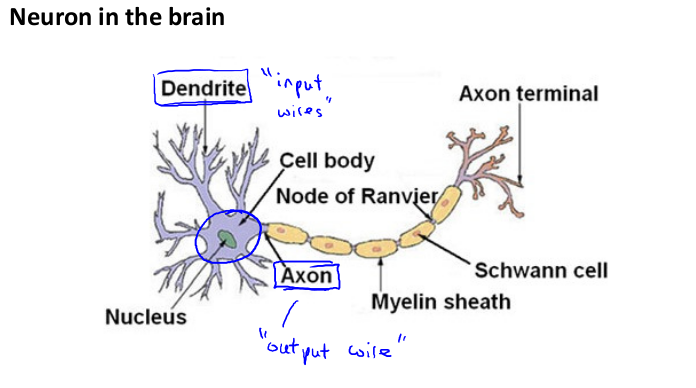
\includegraphics[width=\textwidth]{image/neuron.png}
            \caption{A biological neuron}
            \label{fig:neuron}
        \end{figure}

        Figure \ref{fig:neuron} shows a model of a biological neuron. The \textbf{dendrites} are the wires which receive input signal. The \textbf{axons} output the signal.

        \subsubsection{Neural model: logistic unit}
            In our model:
            \begin{itemize}
                \item Dendrites: input features x\textsubscript{1}, x\textsubscript{2}, \dots, x\textsubscript{n}.
                \item Output: result of hypothesis function.
                \item x\textsubscript{0}: bias unit (:= 1).
                \item Logistic function: $\frac{1}{1+exp(-\theta^T X)}$, referred to as the sigmoid(logistic) \textbf{activation} function.
                \item $\theta$ are referred to as \textbf{weights}.
            \end{itemize}

            Visually, a simplistic representation can be view as 

            \begin{equation}
                [x_0\; x_1\; x_2]\: \rightarrow \: [\:]\: \rightarrow\: h_\theta (x)
                \label{fig:visual-nn-repr}
            \end{equation}


            The input nodes (layer 1, input layer) go into the another node (layer 2), which then outputs to hypothesis function (output layer).

            In this example, we label the intermediate layers of nodes (between the input and output layers) $a^2_0, \dots, a^2_n$: \textbf{activation units}. 
            Definitions:\\

            \fbox{
                $ a_i^{(j)} $ = ``activation of unit i in layer j 
            }\\

            \fbox{
                $\Theta^{(j)}$= matrix of weights controlling function mapping from layer j to layer j+1.
            }\\
          
            If we had one hidden layer, it would look like:

            \[
                \boxed{
                [x_0 \, x_1 \, x_2\, x_3] \:\rightarrow \: [ a_1^{(2)},a_2^{(2)},a_3^{(2)}] \: \rightarrow h_\theta (x)
            }
            \]  
    
            The value for each of the activation node is obtained as follows;

            \[
                a_1^{(2)} = g (\Theta^{(1)}_{10} x_0 + \Theta^{(1)}_{11} x_1 + \Theta^{(1)}_{12} x_2+\Theta^{(1)}_{13} x_3 )
            \] 

            \[
                a_2^{(2)} = g (\Theta^{(1)}_{20} x_0 + \Theta^{(1)}_{21} x_1 + \Theta^{(1)}_{22} x_2+\Theta^{(1)}_{23} x_3 )
            \] 

            \[
                a_3^{(2)} = g (\Theta^{(1)}_{30} x_0 + \Theta^{(1)}_{31} x_1 + \Theta^{(1)}_{32} x_2+\Theta^{(1)}_{33} x_3 )
            \] 

            \[
                h_\Theta(x) = a_1^{(3)} = g (\Theta^{(1)}_{10} a_0 + \Theta^{(1)}_{11} a_1 + \Theta^{(1)}_{12} a_2+\Theta^{(1)}_{13} a_3 )
            \] 

            Essentially, each layer j has its own \textbf{matrix of weights}, $\Theta^{(j)}$.\\
            \fbox{%
                \parbox{\textwidth}{%
                 \textbf{If network has $s_j$ units in layer j and $s_{j+1}$ units in layer j+1,
                then $\Theta^{(j)}$ will be of dimension $s_{j+1} \times (s_j +1)$.
                }
                }%
            }

            The +1 comes from the addition in $\Theta^{(j)}$ of the bias nodes, $x_0$ and $\Theta_0^{(j)}$. 
            
            In the above example, layer 2 has 3 units ( $a_1^{(2)}, a_2^{(2)},a_3^{(2)}$) and layer 1 has 3 units (not including the bias unit). Therefore the weight matrix $\Theta^{(1)}$ which maps layer 1 to layer 2 is of dimension $3\times(3+1)$. 

            Another example: if layer 1 has 2 input nodes and layer 2 has 4 activation nodes- dim ($\Theta^{(1)}$) is going to be 4x3 where $s_j=2$ and $s_{j+1}=4$, so $s_{j+1}\times (s_j +1)=4\times3$.

            \subsubsection{Forward Propagation: Vectorized Implementation}
                Define a new variable: $z_k^{(j)}$ as the parameter for for the logistic function $g(z)$ such that:
                \[
                    a_1^{(2)} = g (z_1^{(2)})
                \] 
                \[
                    a_2^{(2)} = g (z_2^{(2)})
                \] 
                \[
                    a_3^{(2)} = g (z_3^{(2)})
                \] 
              
                Therefore, for layer j=2 and unit k:
                    \[
                        z_k^{(2)} = \Theta^{(1)}_{k, 0} x_0 + \Theta^{(1)}_{k, 1} x_1+ \dots+ \Theta^{(1)}_{k, n} x_n 
                    \]                
                \begin{align*}
                x = \begin{bmatrix}
                        x_0 \\
                        x_1 \\
                        \cdots \\
                        x_n
                    \end{bmatrix} \: &
                z^{(j)} = \begin{bmatrix}
                            z_1^{(j)} \\ 
                            z_2^{(j)} \\
                            \cdots \\
                            z_n^{(j)} \\
                          \end{bmatrix}
                \end{align*}
                We can further generalize by setting $\mathbf{x} = a^{(1)}$ and re-write the equation:
                \begin{equation}
                    z^{(j)} = \Theta^{(j-1)} a^{(j-1)}
                    \label{eq:activation-logistic-z}
                \end{equation}

                Dimension check:  
                \begin{itemize}
                    \item $\Theta^{(j-1)}$ is of dimension $s_j\times (n+1)$.
                    \item a\textsuperscript{(j)} is a column vector with dimension $1\times(j+1)$.
                \end{itemize}

                Thus the logistic function is applied element-wise to \textbf{z}: 
                \begin{equation}
                    a^{(j)} = g (z^{(j)})
                    \label{eq:activation}
                \end{equation}

                We then add the bias unit $a_0^{(j)} = 1$ to the activation matrix. If we propagate forward by one layer in Equation \ref{eq:activation-logistic-z}:
                \begin{equation}
                    z^{(j+1)} = \Theta^{(j)} a^{(j)}
                    \label{eq:formal-activation-x}
                \end{equation}

                The last theta matrix $\Theta^{(j)}$ will have only one row which is multiplied by one column $a^{(j)}$ such that the result is a single scalar.Hence the final hypothesis output is:

                \begin{equation}
                    h_\theta (x) = a^{(j+1)} = g (z^{(j+1)})
                    \label{eq:neural-hypothesis}
                \end{equation}



                


    \subsection{Application - Logic Gate Synthesis}
        We can apply neural networks to predict various logic gates: AND, OR, XOR, NOR.
        The basic graph can be represented as :

        \[
        \begin{bmatrix}
             x_0 \\
             x_1 \\
             x_2
        \end{bmatrix}
        \rightarrow \:
        [\; g (z^{(2)})\;]
        \rightarrow \:
        h_\Theta (x)
        \] 
       



        \subsubsection{AND Gate}
            Let the first theta matrix be:
            \[
                \Theta^{(1)} = [\;\;-30 \;\; 20 \;\; 20 \;\;]
            \] 
          
            Table \ref{tab:AND-gate} outlines the logistic hypothesis output which represents an AND gate: output = 1 $\iff$ ( $x_1=1$ and $x_2 = 1$). The intuition here in choosing the $\Theta$ parameters is that we want the sigmoid function evaluate to be positive only when both x\textsubscript{1} and x\textsubscript{2} are logic 1. Therefore, we assign the bias unit to a large negative value, such that the result of $\Theta x$ is positive only when both the two other weights are added. 

            \begin{table}
                \begin{center}
                    \begin{tabular}[htbp]{|c|c||c|c|}
                        \hline
                        $x_1$ & $x_2$ & z & $h_\Theta (x) = g(z)$ \\
                        \hline
                        \hline
                        0   &   0   &   -30     &   0\\
                        0   &   1   &   -10     &   0\\
                        1   &   0   &   -10     &   0\\
                        1   &   1   &    10     &   1\\
                        \hline
                    \end{tabular}
                \end{center}
                \caption{Truth table of AND gate}
                \label{tab:AND-gate}
            \end{table}


        \subsubsection{OR Gate}

        Similarly, Table \ref{tab:OR-gate} outlines the truth table for the OR function. We pick a parameter matrix:
            \[
                \Theta^{(1)} = [\;\;-10 \;\; 20 \;\; 20 \;\;]
            \] 
          

            \begin{table}
                \begin{center}
                    \begin{tabular}[htbp]{|c|c||c|c|}
                        \hline
                        $x_1$ & $x_2$ & z & $h_\Theta (x) = g(z)$ \\
                        \hline
                        \hline
                        0   &   0   &   -10     &   0\\
                        0   &   1   &    10     &   1\\
                        1   &   0   &    10     &   1\\
                        1   &   1   &    30     &   1\\
                        \hline
                    \end{tabular}
                \end{center}
                \caption{Truth table of OR gate}
                \label{tab:OR-gate}
            \end{table}




        \subsubsection{NOR Gate}

        Similarly, Table \ref{tab:NOR-gate} outlines the truth table for the NOR function. We pick a parameter matrix:
            \[
                \Theta^{(1)} = [\;\;10 \;\; -20 \;\; -20 \;\;]
            \] 
          

            \begin{table}
                \begin{center}
                    \begin{tabular}[htbp]{|c|c||c|c|}
                        \hline
                        $x_1$ & $x_2$ & z & $h_\Theta (x) = g(z)$ \\
                        \hline
                        \hline
                        0   &   0   &    10     &   1\\
                        0   &   1   &   -10     &   0\\
                        1   &   0   &   -10     &   0\\
                        1   &   1   &   -30     &   0\\
                        \hline
                    \end{tabular}
                \end{center}
                \caption{Truth table of NOR gate}
                \label{tab:NOR-gate}
            \end{table}


        \subsubsection{NOT Gate}

        For an inversion, we just need a single parameter x. Table \ref{tab:NOT-gate} outlines the truth table for the NOT function. We pick a parameter matrix:
            \[
                \Theta^{(1)} = [\;\;10 \;\; -20 \;\;]
            \] 
          

            \begin{table}
                \begin{center}
                    \begin{tabular}[htbp]{|c||c|c|}
                        \hline
                        $x$ & z & $h_\Theta (x) = g(z)$ \\
                        \hline
                        \hline
                        0   &    10     &   1\\
                        1   &   -10     &   0\\
                        \hline
                    \end{tabular}
                \end{center}
                \caption{Truth table of NOT gate}
                \label{tab:NOT-gate}
            \end{table}


        \subsubsection{XNOR Gate}
        
        Now, we would like to synthesize the XNOR function (shown in Table \ref{tab:XNOR-gate}. This requires a three level neural network. We can decompose the function XNOR:
            \[
                \overline{ x_1 \oplus x_2} = x_1 x_2 + \overline{x_1}\cdot \overline{x_2}
            \] 
            
            Therefore, in the second layer we will computer the AND and NOR functions then apply OR to the two intermediate output in the third layer. 


            \[
                \Theta^{(1)} = [\;\; -30 \;\; 30 \;\; 20 \;\;]
            \]

            \[
                \Theta^{(2)} = [\;\; -10 \;\; 20 \;\; 20 \;\;]
            \]
            
            
            So:
            \[
                a^{(2)}= g(\Theta^{(1)} \cdot x)
            \]
            \[
                a^{(3)}= g(\Theta^{(2)} \cdot a^{(2)})
            \]
            \[
                h_\Theta (x)= a^{(3)} 
            \] 
   

            \begin{table}
                \begin{center}
                    \begin{tabular}[htbp]{|c|c||c|c||c|}
                        \hline
                    $x_1$   &   $x_2$   &   $a_1^{(2)}$ &   $a_2^{(2)}$ &   $h_\Theta (x)$\\
                    \hline \hline
                    0       &   0       &   0           &   1           &   1 \\
                    0       &   1       &   0           &   0           &   0 \\
                    1       &   0       &   0           &   0           &   0 \\
                    1       &   1       &   1           &   0           &   1 \\
                    \hline
                    \end{tabular}
                \end{center}
                \caption{Truth table of XNOR}
                \label{tab:XNOR-gate}
            \end{table}










            \subsection{Multi-class Classification}
                For multi-class classification, our prediction will be a column vector with each element be of ``whether the current item belongs to the class of that position''. For example, for a 4-class classification, an example output would be:
                \[
                    h_\Theta (x) = [0010]
                \] 

    \section{Neural Networks: Learning}
\subsection{Cost Function}
    Define variables:
    \begin{itemize}
        \item L :total number of layers in the network.
        \item s\textsubscript{l}: number of units (not counting bias unit) in layer l.
        \item K: number of output classes.
    \end{itemize}

    Recall for classifications, we have binary and multi-class:
    \begin{enumerate}
        \item Binary classification:
            \begin{itemize}
                \item y = 0 or 1.
                \item 1 output unit, i.e. $h_\Theta (x) \in \mathbb{R}$.
                \item S\textsubscript{L} = 1; K = 1.
            \end{itemize}
        \item Multi-class classification: 
            \begin{itemize}
                \item $ y \in \mathbb{R}^K$
                \item S\textsubscript{L}= K. K$\geq$3.
            \end{itemize}
    \end{enumerate}

    Recall the cost function for regularized logistic regression in Equation \ref{eq:logistic-cost-function-regularized}, shown below:
    \[
    J(\theta) = \frac{-1}{m} \, \sum_{i=1}^{m}\, [ y^{(i)}\, log\, h_\theta (x^{(i)})\; +\; (1-y^{(i)})\: log\:(\,1-h_\theta(x^{(i)})\,) ] + \frac{\lambda}{2m} \sum_{j=1}^{n} \theta_j^2
    \]

    For neural networks, we will extend Equation \ref{eq:logistic-cost-function-regularized} into a generalized form:
    \begin{equation}
        \begin{aligned}
    J(\Theta) = & \frac{-1}{m} \, \sum\limits_{i=1}^{m}\, \sum\limits_{k=1}^{K}\,[ y_k^{(i)}\, log\, h_\theta (x^{(i)})_k\; +\; (1-y_k^{(i)})\: log\:(\,1-h_\theta(x^{(i)})_k\,) ] \\
    & + \frac{\lambda}{2m} \sum\limits_{l=1}^{L-1}\sum\limits_{i=1}^{s_l}\sum\limits_{j=1}^{s_{l+1}} (\Theta_{j, i}^{(l)})^2
    \end{aligned}
        \label{eq:neural-network-cost-function-regularized}
    \end{equation}

    In the first part of Equation \ref{eq:neural-network-cost-function-regularized}, we added a summation to account for multiple output nodes. 
    Note:
    \begin{itemize}
        \item Double sum adds up logistic regression costs calculated for each cell in the output layer.
        \item Triple sum adds up the squares if all individuals $\Theta$s in the entire network.
        \item The i in the triple sum does not refer to the training example i !
    \end{itemize}

\subsection{Backpropagation Algorithm}
    \begin{itemize}
        \item Backpropagation: neural-network terminology for minimizing cost function.
        \item Gradient Computation: need to computer $J(\Theta)$ and $\frac{\partial }{\partial \Theta^{(l)}_{ij}} J(\Theta)$

    \end{itemize}

    Given a training set \{ $(x^{(1)}, y^{(1)}) \dots (x^{(m)}, y^{(m)})$\}. Set $\Delta^{(l)}_{i,j}=0$ $\forall$ l,i,j.\\
          
    For all training examples t=1:m:
    \begin{enumerate}
        \item Set $a^{(1)} := x^{(t)}$
        \item Perform forward propagation to computer all the nodes ($a^{(l)}$).
        \item Using $y^{(t)}$, compute $\delta^{(L)}=a^{(L)} -y^{(t)} $. (Vectorized deviation of output units to correct values).
        \item Backpropagate the error:
            \[
                \delta^{(l)} = ( (\Theta ^{(l)})^T \delta ^{(l+1)}) .* a^{(l)} .* (1 - a^{(l)})
            \] 
            This equation makes use of the fact that the derivative of the sigmoid function:
            \[
                g'(z^{(l)}) = a^{(l)} .* (1-a^{(l)})
            \] 
        \item Obtain the estimation of gradient ($\nabla J(\Theta)$). Intuitively, $\delta^{(l)}$ is the error for the activation unit in layer l: a\textsuperscript{l}. more formally, the delta values are the derivatives of the cost functions. \\
            It can be shown that 
            \[
                \boxed{
                \frac{\partial}{\partial \Theta^{(l)}_{i,j}} J (\Theta) = a^{(l)}_j \cdot \delta_i^{(l+1)}
            }
            \] 
            Hence, a vectorized implementation of the accumulated gradient  is:
            \[
                \Delta^{(l)} := \Delta^{(l)} + \delta^{(l+1)}(a^{(l)})^T
            \] 
    \end{enumerate}
    We then normalize and add regularization to obtain the gradient:
    \begin{itemize}
        \item $D_{i,j}^{(l)} := \frac{1}{m} (\Delta^{(l)}_{i,j} + \lambda\Theta^{(l)}_{i,j})$, if j $\neq$ 0
        \item $D_{i,j}^{(l)} := \frac{1}{m} \Delta^{(l)}_{i,j}$, if j=0

    \end{itemize}

    And thus $\frac{\partial}{\partial \theta^{(l)}} = D^{(l)}$.
\subsection{Gradient checking}
    \begin{itemize}
        \item Purpose: Eliminates error from escaping. Assuring backpropagation is working as intended.
        \item Approx derivative as:\\
            \[
                \frac{\partial}{\partial \Theta_j} J (\Theta) \approx  \frac{J(\Theta_1, \dots, \Theta_j +\epsilon, \dots, \Theta_n)-J(\Theta_1, \dots, \Theta_j -\epsilon, \dots, \Theta_n)}{2 \epsilon}
            \] 
        \item Compute the gradient approximation and compare with backpropagation(delta vector)
        \item Turn off gradient checking as this is computationally expensive.
    \end{itemize}
    Below is an implementation of gradient checking in MATLAB code:
    \begin{lstlisting}
        epsilon = 1e-4;
        for i = 1:n,
          thetaPlus = theta;
          thetaPlus(i) += epsilon;
          thetaMinus = theta;
          thetaMinus(i) -= epsilon;
          gradApprox(i) = (J(thetaPlus) - J(thetaMinus))/(2*epsilon)
        end;
    \end{lstlisting}

\subsection{Random Initialization}
    \begin{itemize}
        \item Initializing all theta weights to zero does not work. In backpropagation, all nodes will update to the same value repeatedly, creating \textbf{symmetry}. 
        \item Symmetry breaking: initialize to values that range in [-$\epsilon, \epsilon$]
    \end{itemize}


    \section{Advice for Applying Machine Learning}

\subsection{Deciding What to Try Next}
    Potential next steps:
    \begin{enumerate}
        \item Larger training data.
        \item Smaller set of feature.
        \item Additional features.
        \item Polynomial features.
        \item Increase $\lambda$.
        \item Decrease $\lambda$. 
    \end{enumerate}

    Machine Learning Diagnostic: a test to run to gain insight on feasibility of techniques and how to optimize performance. 

\subsection{Evaluating Hypothesis: training/validation/test sets}
    \subsubsection{Motivation with Test sets}
    We want to address the problem of overfitting: fits training examples very well (low error) but fails to generalize and hence not inaccurate on additional data. Thus, to evaluate the true accuracy of hypothesis, we randomly split the data into two sets: a \textbf{training set} (70\%) and a \textbf{test set} (30\%). 
    The procedure :
    \begin{enumerate}
        \item Learn $\Theta$ and minimize $J_{train} (\Theta)$ using the training set
        \item Compute test set error: $J_{test} (\Theta)$. 
            \begin{enumerate}
                \item For linear regression: 
                    \[
                    J_{test} (\Theta) =  \frac{1}{2m_{test}} \sum_{i=1}^{m_{test}} (h_\theta(x_{test}^{(i)}) - y_{test}^{(i)} )^2
                    \]
                \item For logistic regression:
                    \[
                        J (\theta) = \frac{-1}{m_{test}} \sum_{i=1}^{m_{test}} (y^{(i)}_{test} log(h_{\Theta} ( x^{(i)}_{test}) + (1-y^{(i)}_{test}) log(1-h_{\Theta} ( x^{(i)}_{test}) )
                    \] 
                \item For classification, we first calculate the misclassification error. 
                    \begin{equation}
                        err (h_{\Theta} (x), y) = 
                        \begin{cases}
                            1 &\quad \text{if } (h_\Theta (x) \geq 0.5 \: \& \: y=0)\text{ or } (h_\Theta (x) \leq 0.5 \:\&\:  y=1) \\
                            0 &\quad \text{if otherwise. }  \\
                        \end{cases}
                        \label{eq:misclassification-error}
                    \end{equation}

                    The average test error is thus:
                    \begin{equation}
                        \text{Test error} = \frac{1}{m_{test}} \sum_{i=1}^{m_{test}} err (h_{\Theta} (x), y)
                        \label{eq:classification-test-error}
                    \end{equation}

            \end{enumerate}
    \end{enumerate}


    \subsubsection{Polynomial features: Train/Validation/Test model}
        \begin{itemize}
            \item Computed cost is less than the generalization error: We trained our data on the training set to obtain $\Theta$ with different degrees of polynomial (d). We then choose d based on minimizing the test set.
            \item Problem: $J_{test} (\Theta)$ is likely to be an optimistic generalization error, since the parameter d is fit to the test data set.
            \item Solution: break down dataset into three sections:
                \begin{enumerate}
                    \item Training set (60\%).
                    \item Cross-validation set (20\%).
                    \item Test set (20\%).
                \end{enumerate}

        \end{itemize}

        Procedure:
        \begin{enumerate}
            \item Optimize the parameters in $\Theta$ using the training set for each polynomial degree.
            \item Find the polynomial degree d with the least error using the cross validation set.
            \item Estimate the generalization error using the test set with $J_{test}(\Theta^{(d)})$, (d = theta from polynomial with lower error);
        \end{enumerate}

        This way, the degree of the polynomial d has not been trained using the test set.
    

    
        
\subsection{Diagnosing Bias vs Variance}
    \begin{itemize}
        \item Degree of polynomial (d) and underfitting (high bias) / overfitting (high variance).
        \item Training errors tend to decrease as d increases. 
        \item Cross validation error tends to form a convex curve with a minimum point. 
    \end{itemize}

    Therefore, the key to distinguish between bias and variance is summarized in Figure \ref{fig:error-bias-variance}. 
    \begin{figure}[htbp]
        \centering
        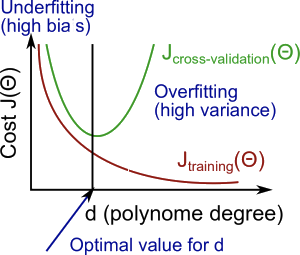
\includegraphics[width=0.5\textwidth]{image/error-bias-variance.png}
        \caption{Error cost of cross-validation and training over degree of polynomial}
        \label{fig:error-bias-variance}
    \end{figure}

    \begin{enumerate}
        \item \textbf{High bias (underfitting)}: both $J_{train} (\Theta)$ and $J_{CV} (\Theta)$ will be high. Thus: $J_{train} (\Theta) \approx J_{CV} (\Theta)$
        \item  \textbf{High variance (overfitting)}: \emph{Low} $J_{train} (\Theta)$ and \emph{high} $J_{CV} (\Theta)$. Thus: $J_{train} (\Theta) <<  J_{CV} (\Theta)$

    \end{enumerate}

\subsection{Regularization and bias and variance}
    \begin{itemize}
        \item Large $\lambda$ (lower significance of $\Theta$, heavy penalization so $h_\theta \approx 0$): high bias, underfit. 
        \item Small $\lambda$ (high significance of $\Theta$): high variance, overfit. 
    \end{itemize}

    Procedure to pick the right $\lambda$:
    \begin{enumerate}
        \item Create list of lambda. 
        \item Iterate through $\lambda$s and learn/obtain $\Theta$. 
        \item Compute cross-validation error ($J_{CV} (\Theta) $) using the learned $\Theta$ \textbf{without regularization} (i.e. $\lambda = 0$)
        \item Select the best lambda and Theta pair and verify on test set. (Compute $J_{test} (\Theta)$.
    \end{enumerate}
\subsection{Learning Curves}
    Plotting error over number of training examples. 
    \subsubsection{High bias}
        \begin{enumerate}
            \item Low training set size: low $J_{train}$ and high $J_{CV}$.
            \item Large training set size: high $J_{train}$ and high $J_{CV}$.
        \end{enumerate}

        Getting more training data will not help. 
        \begin{figure}[htbp]
            \centering
            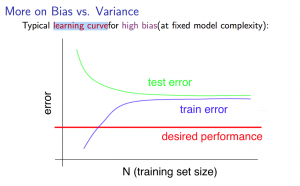
\includegraphics[width=\textwidth]{image/learning-curve-high-bias.png}
            \caption{Learning curve for high bias}
            \label{fig:learning-curve-high-bias}
        \end{figure}
    
    \subsubsection{High variance}
        \begin{enumerate}
            \item Low training set size: low $J_{train}$ and high $J_{CV}$.
            \item Large training set size: $J_{train}$ increases and $J_{CV}$ decreases.
        \end{enumerate}

        Getting more training data will help. 
        \begin{figure}[htbp]
            \centering
            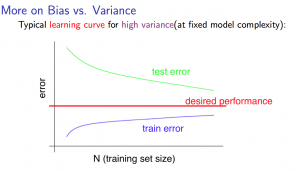
\includegraphics[width=\textwidth]{image/learning-curve-high-variance.png}
            \caption{Learning curve for high variance}
            \label{fig:learning-curve-high-variance}
        \end{figure}

\subsection{Summary}
    \begin{enumerate}
        \item Getting more training examples: Fixes high variance
        \item Trying smaller sets of features: Fixes high variance
        \item Adding features: Fixes high bias
        \item Adding polynomial features: Fixes high bias
        \item Decreasing $\lambda$: Fixes high bias
        \item Increasing $\lambda$: Fixes high variance.
    \end{enumerate}
\subsection {Neural Networks}
    \begin{enumerate}
        \item Small neural network: fewer parameters $\implies$ prone to underfitting, but computationally cheaper. 
        \item Large neural network: more parameters $\implies$ prone to overfitting, computationally expensive. Use regularization to address overfitting. 
    \end{enumerate}
    

    \section{Machine Learning System design}

\subsection{Prioritizing what to work on: Spam Classification Example}
    \begin{itemize}
        \item Supervised learning.
        \item \textbf{x} = features of email (words indicative of spam).
        \item y = 1 (spam) or 0 (not spam). 
        \item In practise, we take the most frequent n words (10000 to 50000) in training set to use as elements in x. 
    \end{itemize}

    Potential next steps:
    \begin{enumerate}
        \item Collect lots of data.
        \item Develop sophisticated features, e.g. for email routing information, message body, etc. 
        \item Sophisticated algorithms.
    \end{enumerate}

\subsection{Error Analysis}
    \subsubsection{Recommended Approach}
        \begin{itemize}
            \item Start with simple algorithm that can be implemented quickly. Implement and test on \emph{Cross-validation data}. 
            \item Plot learning curves to decide if more data or more features will help. 
            \item Error analysis: Manually examine errors from the examples in \emph{cross-validation} set. Observe any systematic trend. 
        \end{itemize} 

    \subsubsection{Error Analysis}
        Questions to ask:
        \begin{enumerate}
            \item What type of email it is.
            \item What cues (features) do you think would have helped the algorithm to classify them correctly. 
        \end{enumerate}

    \subsubsection{The importance of numerical evaluation}
        \begin{itemize}
            \item Should discount/discounts/discounted/discounting be treated as the same word? 
                \begin{itemize}
                    \item Use "stemming" software, e.g. \emph{Porter Stemmer}
                \end{itemize}
            \item Error analysis might not help. Instead, try and see it it works.
            \item Need metric (numerical evaluation) of algorithm to evaluate performance. E.g. cross validation error.
        \end{itemize}
\subsection{Error Metrics for Skewed Classes}
    \subsubsection{Motivation} 
        Consider case for cancer classification. If we get 1\% error on the test set, i.e. 99\% diagnoses are correct. However, only 0.5\% of patients have cancer in the first place. Is the 1\% error a good evaluation?
        Furthermore, consider the example prediction algorithm:
        \begin{lstlisting}
            function y = predictCancer(x)
                y=0; %ignore x!
            return
        \end{lstlisting}

        Regardless of the dataset, the hypothesis will always predict y=0. 
    \subsubsection{Precision/Recall}

        \begin{table}[htbp]
                \begin{center}
                     \begin{tabular}{|c||c|c|c|}
                         \hline
                         & Actual &   1               &   0  \\
                         \hline
                         \hline
                         Prediction &1               &   True positive   &   False positive  \\
                         \hline 
                         & 0               &   False negative  &   True negative   \\
                         \hline
                    \end{tabular}
                 \caption{Truth Table}
                 \label{tab:truth-table}
             \end{center}
         \end{table}


        We can thus define two measures of accuracy:
        \begin{equation}
            \mathbf{precision} = \frac{\text{True pos}}{\text{No. of predicted pos}} = \frac{\text{True pos}}{\text{True pos + False pos}}
            \label{eq:precision}
        \end{equation}

        \begin{equation}
            \mathbf{recall} = \frac{\text{True pos}}{\text{No. of actual pos}} = \frac{\text{True pos}}{\text{True pos + False neg}}
            \label{eq:recall}
        \end{equation}

        \fbox{
        Convention: Define y=1 in presence of \emph{rare class} that we want to detect.
    }

\subsection{Trading off Precision and Recall}
Recall that for logistic regression, we have the hypothesis $0 \leq h_\theta(x) \leq 1$. Note that earlier we set the threshold to be 0.5. Now we can set the threshold higher (e.g, 0.8 for a more confident prediction), or lower (e.g. 0.3 for a greater coverage).\\ 
    \par Consider two use cases:
    \begin{enumerate}
        \item Suppose we want to predict y=1 (cancer) only if we are very confident: We will set the threshold to be high.\\
            High precision, low recall.
        \item Suppose we want to avoid missing too many cases of cancer (avoid false negatives): We will set the threshold to be low.\\
            High recall, low precision.
    \end{enumerate}

    \subsubsection{F\textsubscript{1} score}
        Now that we have two metrics, precision and recall, we need a method to combine the two into a single metric evaluation for comparison purposes. An initial step may be to use the arithmetic mean. However, this can be inaccurate when either precision or recall is extremely high and the other extremely low. The mean will yield a somewhat high value. We need a better metric. Here we propose the F\textsubscript{1} score:
        \begin{equation}
            F_1 = 2 \: \frac{PR}{P+R}
            \label{eq:f1-score}
        \end{equation}
    \subsubsection{Large Data Rationale}
    At some point, we will need to acquire more data. A larger dataset is useful when $x\in\mathbb{R}^{n+1}$ has sufficient information to predict y accurately. 
    A useful mental test is: given the input x, can a human expert confidently predict y?

    When we use a learning algorithm with many parameters, e.g. logistic regression, linear regression with many features; neural network with many hidden units. This ensures a low bias algorithm. Therefore $J_{train} (\Theta)$ will be small. 
    \par Now, we can then use a large training set (which is unlikely to overfit) and ensure low variance. In such case, $J_{train} (\Theta) \approx J_{test}(\Theta)$, which makes the test error low. 


    \section{Support Vector Machine}

\subsection{Optimization Objective}
    \subsubsection{Alternative View of Logistic Regression}
        \[
            h_\theta(x) = \frac{1}{1 + e^{-\theta^T x}} 
        \] 

        If y = 1, we want $h_\theta(x) \approx 1$, $\theta^T x >> 0$. 
        \par If y = 0, we want $h_\theta(x) \approx 0$, $\theta^T x << 0$
        
        Cost of example:
        \[
            \boxed{
        y\;log\;h_\theta(x)\:\;+\:\;(1-y)\;log(1-h_\theta(x)))\;=\;-y\;log\;\frac{1}{1\;+\;e^{-\theta^Tx}}\;-\;(1-y)\;log\;(1-\frac{1}{1+\;e^{\theta^T\;x}})
            }
        \] 

        Consider the two terms in the above equation, where now we replace the cost with a straightened two-section curve:
 
        \begin{figure}[htbp]
            \centering
            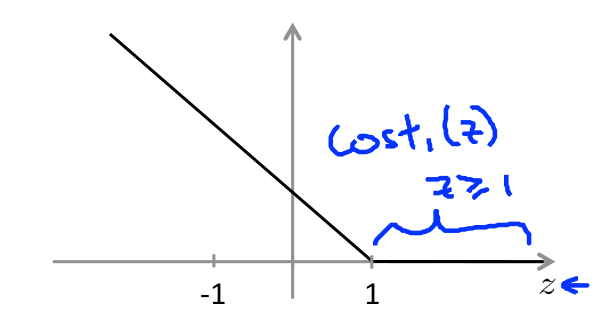
\includegraphics[width=0.5\textwidth]{image/SVM-cost1.png}
            \caption{SVM cost\textsubscript{1}}
            \label{fig:SVM-cost1}
        \end{figure}

       \begin{figure}[htbp]
            \centering
            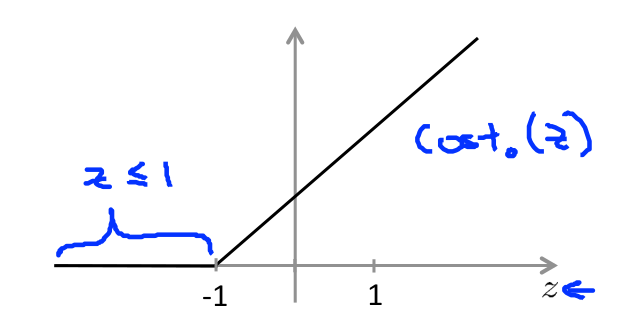
\includegraphics[width=0.5\textwidth]{image/SVM-cost0.png}
            \caption{SVM cost\textsubscript{0}}
            \label{fig:SVM-cost0}
        \end{figure}

        \begin{enumerate}
            \item If y=1 , want $h_\theta(x) \approx 1$, $\theta^T x >> 0$. Here we label the curve as cost\textsubscript{0} (z), as shown in Figure \ref{fig:SVM-cost1}.
            \item If y = 0, we want $h_\theta(x) \approx 0$, $\theta^T x << 0$. Here we label the curve as cost\textsubscript{1}(z), as shown in Figure \ref{fig:SVM-cost0}..
        \end{enumerate}

        \subsubsection{Support Vector Machine}
        Recall logistic regression has the form as in Equation \ref{eq:logistic-cost-function-regularized}, shown below in an alternate form (taking the negative sign into the summation):
    \[
J(\theta) = \frac{1}{m} \, \sum_{i=1}^{m}\, [ y^{(i)}\, -log\, h_\theta (x^{(i)})\; \; -(1-y^{(i)})\: log\:(\,1-h_\theta(x^{(i)})\,) ] + \frac{\lambda}{2m} \sum_{j=1}^{n} \theta_j^2
    \] 

    The Support Vector Machine has a similar form as logistic regression, with a few conventions that differ from its logistic regression counterpart:
    \begin{enumerate}
        \item Remove scaling term ($\frac{1}{m}$). Note that this does not change the final result of minimized $\theta$.
        \item The logistic regression has the form: $A + \lambda B$; the SVM has the form $CA + B$. This is just a different way of parametrizing tradeoffs. Note here C behaves similarly to $\frac{1}{\lambda}$.
    \end{enumerate}

    Therefore, the SVM hypothesis can be expressed in Equation \ref{eq:svm}.

    \begin{equation}
        \underset{\theta}{min}\: C \sum_{i=1}^{m}\, [ y^{(i)}\, cost_1 (\theta^T x^{(i)}) + \; (1-y^{(i)})\:cost_0 (\theta^T x^{(i)})] + \frac{1}{2} \sum_{j=1}^{n} \theta_j^2
        \label{eq:svm}
    \end{equation}

    The hypothesis
    \[
        h_\theta (x) = 
        \begin{cases}
       1 &\quad \text{if } \theta^T x \geq 0 \\
       0 &\quad \text{if otherwise. }  \\
        \end{cases}
    \]

\subsection{Large Margin Intuition}
Recall in Figure \ref{fig:SVM-cost1} and \ref{fig:SVM-cost0}, we re-defined the function. Herein, we have shifted our threshold to z=1 and z=-1 respectively for predicting y = 1 and 0, respectively. This is different from previous threshold of 0 for logistic regression. We are more conservative in our predictions here, by using the 2 new segment cost functions, cost\textsubscript{1}($\theta^T x^{(i)}$) and cost\textsubscript{0}($\theta^T x^{(i)}$). 
    \subsubsection{SVM Decision Boundary}
    Suppose we set C to be a large number, e.g. 10000. Under the minimization objective, we will be highly motivated to pick a $\theta$ such that the first term is close to zero, thus discarding the first term. 
    The original equation will then be reduced effectively to 
    \[
        \underset{\theta}{min} \: \frac{1}{2} \sum_{j=1}^{n} \theta_j^2
    \] 
    
    such that 
    \[
    \theta^T x^{(i)}
         \begin{cases}
       \geq 1 &\quad \text{if } y^{(i)} = 1\\
       \leq -1 &\quad \text{if } y^{(i)} = 0  \\
        \end{cases}
    \] 

    \subsubsection{Large Margin Classifier}
    The Support Vector Machine is also known as the Large Margin Classifier. The word margin refers to the distance between the boundary and the data points. SVM will try to maximize the distance, as seen in Figure \ref{fig:SVM-decision-boundary-margin}. 
    \begin{figure}[htbp]
        \centering
        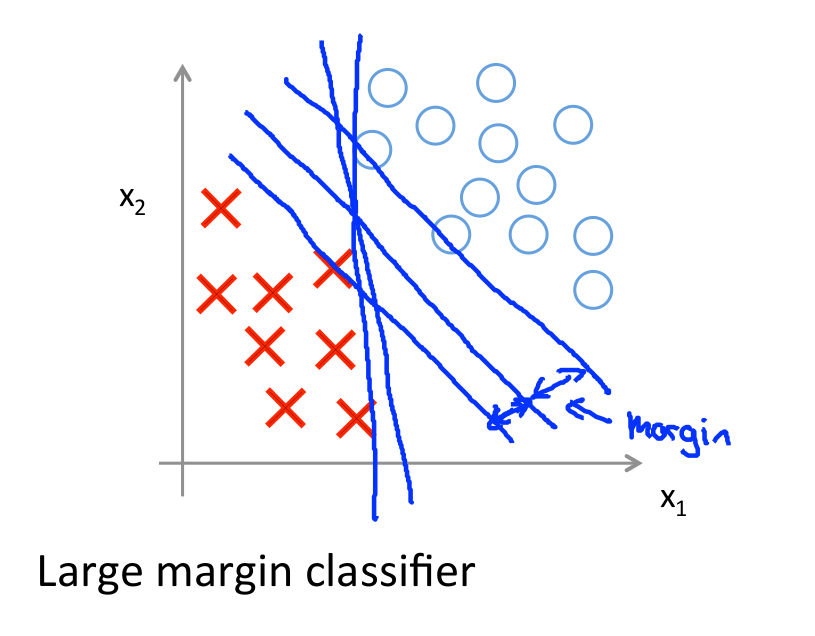
\includegraphics[width=0.5\textwidth]{image/SVM-decision-boundary-margin.png}
        \caption{SVM Decision Boundary: Linearly Separable Case}
        \label{fig:SVM-decision-boundary-margin}
    \end{figure}

        When C is too large (similar to a small $\lambda$), then we get decrease the power of the margin margin classifier, and the algorithm will fit too well to outliers. 

\subsection{Kernels}
    \subsubsection{Non-linear decision boundary}
    For a non-linear decision boundary problem (as shown in Figure \ref{fig:non-linear-decision-boundary-problem}), we have:
        \[
            h_{\theta} = 
            \begin{cases}
                1,                      &\quad \text{if } \theta_0 x + \theta_1 x_1 + \dots \geq 0 \\
                0,                      &\quad \text{otherwise } \\
            \end{cases}
        \] 

        This can be written as 
        \[
        \theta_0 x + \theta_1 f_1 + \theta_2 f_2+ \theta_3 f_3 + \dots
        \] 
        , where 
        \[
            f_1 = x_1, f_2 = x_2, f_3 = x_1x_2, f_4 = x_1^2, f_5 = x_2^2 \dots
        \] 


        However, high order polynomials are expensive. Is there a better choice of features $f_i$'s?

        \begin{figure}[htpb]
            \centering
            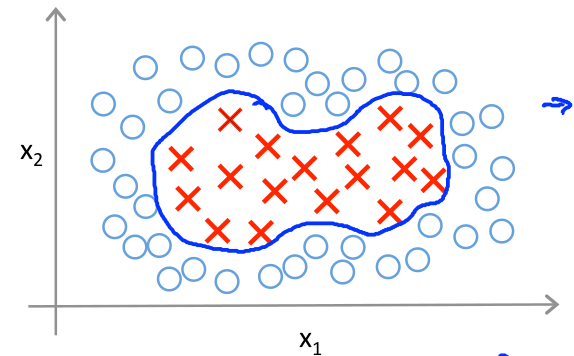
\includegraphics[width=0.5\textwidth]{image/non-linear-decision-boundary.png}
            \caption{Nonlinear decision boundary problem}
            \label{fig:non-linear-decision-boundary-problem}
        \end{figure}

    \subsubsection{Kernel}
    Given $x$, compute new feature depending on proximity to landmarks $l^{(1)}, l^{(2)}, l^{(3)}$. This can be illustrated in Figure \ref{fig:landmark}. 

    \begin{figure}[htbp]
        \centering
        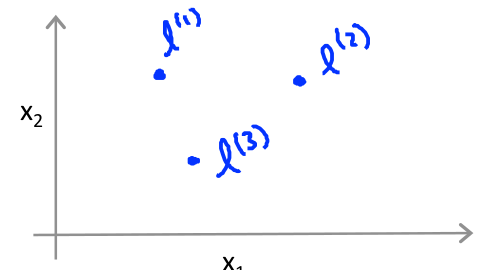
\includegraphics[width=0.5\textwidth]{image/landmark.png}
        \caption{Kernel and landmark illustration}
        \label{fig:landmark}
    \end{figure}

    We then compute the features $f_i = kernel(x, l^{(i)})$ as follows: 
    \begin{equation}
        f_i = \text{similarity}(x, l^{(i)}) = exp ( - \frac{\| x-l^{(i)}\|^2}{2\sigma^2})
        \label{eq:guassian-kernel}
    \end{equation}
    This is a specific type of kernel, namely, the \emph{Gaussian kernel}.

    \subsubsection{Kernels and Similarity} 
    Note: The term $\| x-l^{(i)} \|$ in \ref{eq:guassian-kernel} can also be written as: $\sum_{j=1}^{n} (x^j - l^{(i)}_j)^2$. We can analyze the term in two scenarios:
    \begin{enumerate}
        \item If $x\approx l^{(i)}$, then $\| x-l^{(i)} \|\approx 0$, consequently $f_i \approx 1$.
        \item If $x$ is far from $l^{(i)}$, then $\| x-l^{(i)} \|$ large, consequently $f_i \approx 0$.
    \end{enumerate}

    Each landmark $l^{(i)}$ defines a new feature $f_i$, where the function approaches one when x is close to the landmark, and approaches zero otherwise.

    The function can be visualized in Figure \ref{fig:guassian-kernel-plot}. Note that as the variance ($\sigma$) increases, f falls from the peak (1) slower.
   \begin{figure}[htpb]
       \centering
       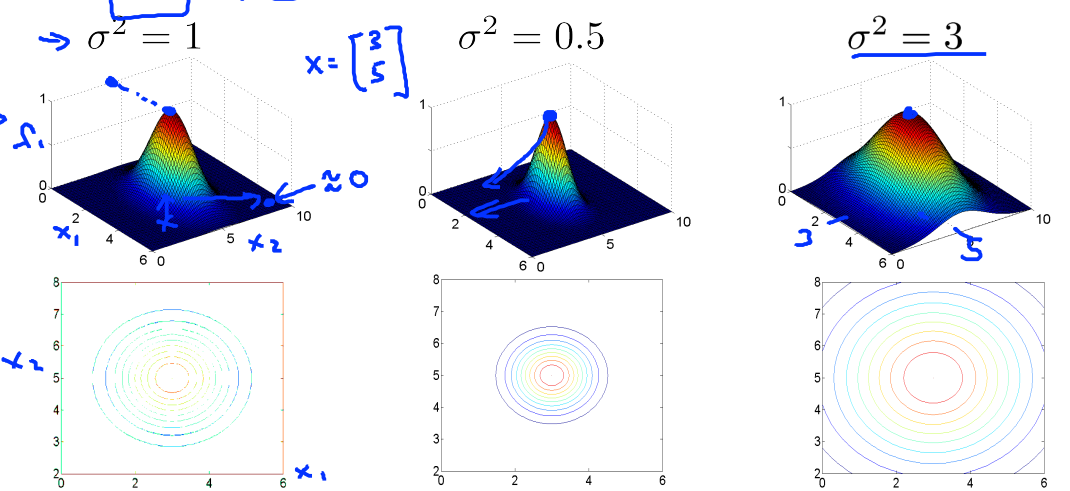
\includegraphics[width=0.7\textwidth]{image/guassian-kernel-plot.png}
       \caption{Guassian Kernel 3D plot}
       \label{fig:guassian-kernel-plot}
   \end{figure} 
   \subsubsection{Choosing Landmark}
   A natural question arises: \emph{Where do we get $l^{(i)}$?} 
   \par Recall from \ref{eq:guassian-kernel}, given x we can compute a feature (f\textsubscript{i}) as the similarity between the point and the landmark.   


   We predict y = 1, when 
   \[
       \sum_{i}^{n} \theta_i f_i \geq 0
   \] 
   In practise, $\theta_0$ is chosen to be negative, where $\theta_i, (i\neq 0)$ are chosen to be some non-negative constants. As such, the closer $x_i$ is to each $l_i$, $f_i$ will tend to 1, thus making the term $\theta_i f_i$ some positive number. We then take the sum of "weighted proximities to each landmark", and make the decision on y. 

   \par Observe Figure \ref{fig:landmark-selection}, where the markings of datasets we want is in blue, and red are the ones that we discard. Our goal is to guess what data belongs to our identification. Hence, we want to identify $x$ that is close to our training examples. 

   \begin{figure}[htpb]
       \centering
       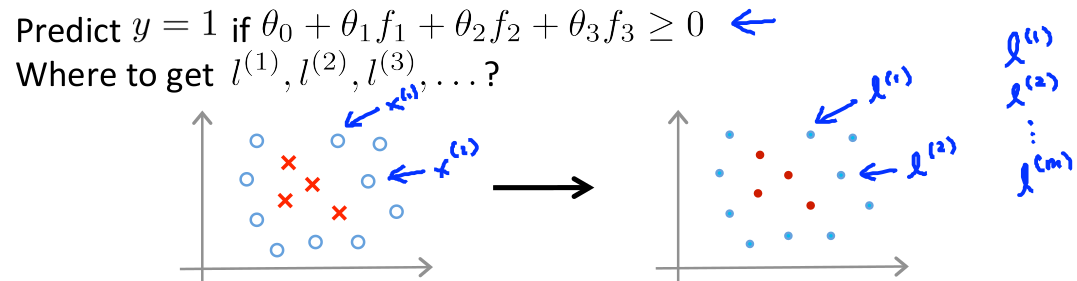
\includegraphics[width=0.7\textwidth]{image/landmark-selection.png}
       \caption{Landmark and Training dataset}
       \label{fig:landmark-selection}
   \end{figure}

   \par Comparing the above two paragraphs, it follows naturally that we should choose the training examples as our landmarks. Thus features are a measure of \emph{proximity to training examples}, given an $x$.
   \subsubsection{SVM with Kernels}
        A summary of our setup:
        \begin{itemize}
            \item Given training examples:  $(x^{(i)}, y^{(i)})$, i = $1\dots m$.
            \item Select landmarks:         $l^{(i)} = x^{(i)}$
            \item Given example $x$:   compute features $f_i = similarity(x, l^{(i)})$. \\
                For training example $(x^{(i)}, y^{(i)})$, where $x^{(i)} \in \mathbb{R}^{n+1} \; (0 \dots n)$. We can compute the feature vector $f^{(i)} \in \mathbb{R}^{m+1}$, where $m$ is the number of landmarks (training examples).
                \[
                f^{(i)} = \begin{bmatrix}
                    f_0^{(i)}   \\
                    f_1^{(i)}   \\
                    f_2^{(i)}   \\
                    \vdots      \\
                    f_i^{(i)}   \\
                    \vdots      \\
                    f_m^{(i)}
                            \end{bmatrix}
                \] 
                \begin{enumerate}
                    \item $f_0^{(i)} = 1$ by default.
                    \item $f_i^{(i)} = 1$ by design (check Equation \ref{eq:guassian-kernel}; similarity of $x^{(i)}$ to $l^{(i)}= x^{(i)}$ is 1).
                \end{enumerate}
                    
        \end{itemize}


        Formally:
        \begin{enumerate}
            \item \textbf{Hypothesis}: Given $x \in \mathbb{R}^{n+1}$, compute features $f \in \mathbb{R}^{m+1}$. \\
                Predict "y = 1", if $\theta^T f  = \sum_{i=0}^{m} \theta_i f_i \geq 0$
            \item \textbf{Training}: 
                \[
        \underset{\theta}{min}\: C \sum_{i=1}^{m}\, [ y^{(i)}\, cost_1 (\theta^T f^{(i)}) + \; (1-y^{(i)})\:cost_0 (\theta^T f^{(i)})] + \frac{1}{2} \sum_{j=1}^{m} \theta_j^2
            \] 
                Remarks: 
                \begin{itemize}
                    \item The above equation is similar to \ref{eq:svm}.
                    \item We calculate the cost based on $\theta$ and $f^{i}$.
                    \item In the second summation, $n=m$; number of features=number of training sets.
                \end{itemize}
            \item \textbf{Implementation Note}
                \begin{itemize}
                    \item $\sum_{j=1}^{m} \theta_j^2 = \theta^T \theta; 
                            \theta = \begin{bmatrix}
                            f_0     \\
                            f_1     \\
                            f_2     \\
                            \vdots  \\
                            f_m     \\
                                    \end{bmatrix}$ 
                    \item Can also scale $\theta$, i.e. $\theta^T M \theta$.
                    \item $M$ increases computation efficiency.
                \end{itemize}
        \end{enumerate}

        
    \subsubsection{SVM Parameters}
    We have two parameters: C and $\lambda$: \\
    \par \textbf{C}= $\frac{1}{\lambda}$:
    \begin{enumerate}
        \item Large C (small $\lambda$): lower bias, higher variance.
        \item Small C (large $\lambda$): Higher bias, low variance.
    \end{enumerate}

    \par \textbf{$\sigma^2$}: (see Figure \ref{fig:guassian-kernel-plot})
    \begin{enumerate}
        \item Large $\sigma^2$: (features $f_i$ vary more smoothly) higher bias, lower variance.
        \item Small $\sigma^2$: (changes abruptly) lower bias, higher variance.
    \end{enumerate}

\subsection{Using an SVM}
    \begin{itemize}
        \item Use SVM software package (e.g. linlinear, libsvm, $\dots$) to sole for parameters $\theta$
        \item Specification: 
            \begin{enumerate}
                \item Parameter C.
                \item Kernel (similarity function) 
                        \begin{itemize}
                            \item No kernel ("linear kernel"): predicts "y=1" if $\theta^T x \geq 0$.
                            \item Guassian kernel: $f_i = exp ( - \frac{\| x-l^{(i)}\|^2}{2\sigma^2})$, need to choose $\sigma^2$, perform feature scaling.
                        \end{itemize}
            \end{enumerate}
        \item Other choices of kernel: not all similarity functions make valid kernels. Need to satisfy \emph{Mercer's Theorem} for convergence. Off-the-shelf kernels:
            \begin{itemize}
                \item Polynomial kernel
                \item String kernels (text)
                \item Chi-squared kernel
                \item Histogram intersection kernel
            \end{itemize}
    \end{itemize}

\subsection{Multiclass Classification}
For illustration, see Figure \ref{fig:multi-class-svm}. Many SVM packages have built-in functionalities. Otherwise, we can implement using one-vs-all method:
\begin{itemize}
    \item Train K SVMs, each distinguish $y=i, \forall i = 1, 2, \dots K$ from the rest.
    \item Get $\theta^{(1)}$, $\theta^{(2)}$, $\theta^{(3)}$, $\dots$, $\theta^{(K)}$.
    \item Pick class $i$ with largest $(\theta^{(i)})^T x$.


\end{itemize}
\begin{figure}[htpb]
    \centering
    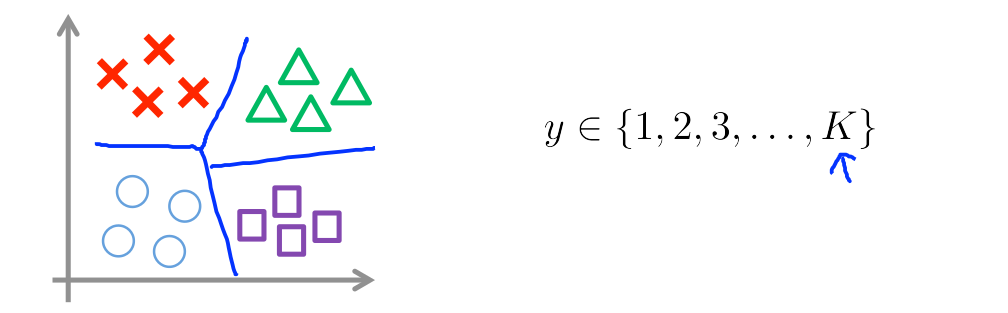
\includegraphics[width=0.5\textwidth]{image/multi-class-svm.png}
    \caption{Multiclass SVM}
    \label{fig:multi-class-svm}
\end{figure}


\subsection{Logistic Regression v.s. SVMs}
    Let:
    \begin{itemize}
        \item $n$ = number of features ($x \in \mathbb{R}^{n+1}$)
        \item $m$ = number of training examples.
    \end{itemize}

    \begin{enumerate}
        \item If $n \gg m$: use logistic regression, or SVM without a kernel (linear kernel).
        \item If $n < m$: use SVM with Guassian Kernel.
        \item IF $n \ll m$: Create/add more features, then use logistic regression or SVM without a kernel.
        \item  Neural network: likely to work in all cases, but may be slower to train.
    \end{enumerate}
    

    \section{Clustering}
\subsection{Unsupervised learning introduction}
    Sometimes we do not have a training set with defined labels (results); therefore, we need to find some structure from the training set.
    \textbf{Clustering} is one way to do so, by grouping close data points together.


    Applications of clustering:
    \begin{itemize}
        \item Market segmentation.
        \item Social network analysis.
        \item Organize computer clusters.
        \item Astronomical data analysis.
    \end{itemize}

\subsection{K-means algorithm}
    K-means algorithm performs clustering by defining a "centroid" for each cluster and improve the accuracy of centroids through minimizing the total squared distances from the centroid to all points in the particular cluster.

    \begin{enumerate}
        \item Input: 
            \begin{itemize}
                \item $K$ (number of clusters).
                \item Training set ${x^{(1)}, x^{(2)},x^{(3)}, \dots x^{(m)})}$. $x^{(i)} \in \mathbb{R}^n$ (We drop the $x_0 = 1$ convention.
            \end{itemize}
        \item \textbf{Algorithm} The K-means algorithm has three main steps:
            \begin{enumerate}
                \item \textbf{Initialization}: Initialize cluster centroids (random).
                \item \textbf{Cluster Assignment}: (Loop: for all data points $x$) assignment of each data point into a cluster, depending on the proximity to the cluster centroid.
                \item  \textbf{Move Centroid}: (Loop: for all clusters) refine the centroid of each cluster by taking the mean location of all data points for an individual cluster.
            \end{enumerate}
            \begin{algorithm}[H]
            \caption*{K-means Algorithm}
            \begin{algorithmic}
                \STATE  Randomly initialize $K$ cluster centroids $\mu_1, \mu_2, \dots, \mu_K \in \mathbb{R}^n$ 
                \STATE \textbf{Repeat} \{
                \bindent
                \FOR{i=1 to m}
                \STATE $c^{(i)} := k$, s.t. $\min_{k} \| x^{(i)} - \mu_k \| ^2 $ \\
                \COMMENT {\textbf{Cluster assignment}: index ($ 1 \dots K$) of cluster centroid closest to $x^{(i)}$}
                \ENDFOR
                \eindent
                \\ 
                \bindent
                \FOR{k= 1 to K}
                \STATE $\mu_k$ := mean of points assigned to cluster k \\
                \COMMENT{\textbf{Move centroid}}
                \ENDFOR
                \eindent

            \STATE \}
            \end{algorithmic}
            \end{algorithm}
        \item K-means for non-separate clusters: sometimes the clusters are not well defined (separated enough). The algorithm will still produce clustering based on the proximity. An example is the \textbf{T-shirt sizing problem} (See Figure \ref{fig:t-shirt-sizing}) : for a given set of weight-height distribution from market survey, how many sizes should the manufacturer produced (S, M, L) or (XS, S, M, L, XL)?
    \end{enumerate}
    \begin{figure}[htpb]
        \centering
        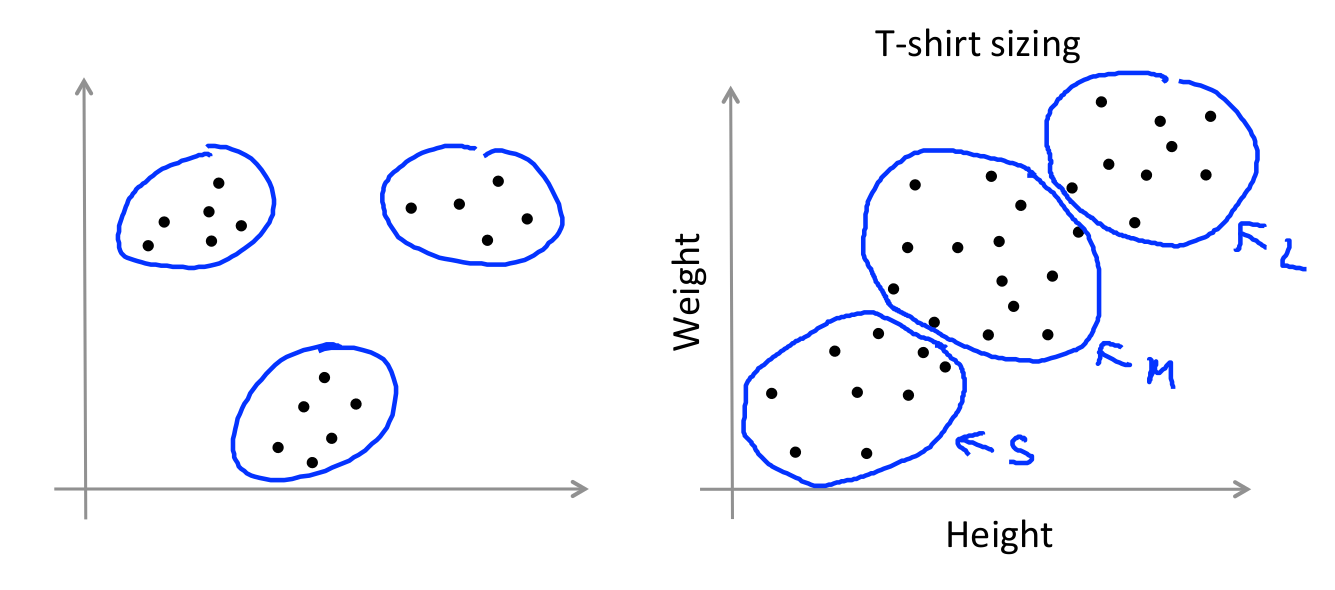
\includegraphics[width=0.8\textwidth]{image/t-shirt-sizing.png}
        \caption{Non-separated clusters: T-shirt sizing}
        \label{fig:t-shirt-sizing}
    \end{figure}
\subsection{Optimization Objective}
    \begin{enumerate}
        \item $c^{(i)}$ = \textbf{index}of cluster (1, 2, $\dots K$) to which example $x^{(i)}$ is currently assigned.
        \item $\mu_k$ = cluster centroid k. [Coordinate $\mu_k \in \mathbb{R}^n$]
        \item $\mu_{c^{(i)}}$ = cluster centroid of cluster to which example $x^{(i)}$ has been assigned.
        \item \textbf{Optimization objective}: \\
            \begin{equation}
                \min_{ \{c^{(i)}\}, \{\mu_k\} } J ( \{c^{(i)}\}, \{\mu_k\} )
                \label{eq:k-means-objective}
            \end{equation}
           \begin{equation}
                J ( \{c^{(i)}\}, \{\mu_k\} ) = \frac{1}{m} \sum_{i=1}^{m} \| x^{(i)} - \mu_{c^{(i)}} \|^2
               \label{eq:k-means-cost}
           \end{equation} 

           Note:
           \begin{enumerate}
               \item The first for loop in the algorithm (i) minimizes $J(\dots)$ with respect to $c^{(i)}$ and holds $\mu_k$ constant.
               \item The second for loop in the algorithm (k) minimizes $J(\dots)$ with respect to $\mu_k$ and holds $c^{(i)}$ constant.
           \end{enumerate}

    \end{enumerate}
\subsection{Random Initialization}
    Rules:
    \begin{enumerate}
        \item $K$ < m (number of training examples).
        \item Randomly pick $K$ training examples.
        \item Set $\mu_k$ to the K examples chosen in the previous step.
    \end{enumerate}

    There might be different clustering based on different initial random selection. Therefore one can run the K-means algorithm multiple times (100), each with a different random initialization (selection of examples as initial centroids). Compute all cost function (distortion), then pick the one that gives the lowest cost J.

\subsection{Choosing the number of clusters ($K$)}
    Sometimes it is ambiguous how many clusters there are, e.g. could be 2 or 4. One method of determining the number of clusters is the \emph{Elbow method}. We compute the cost and vary $K$- we will usually see a sharp drop in cost at the star, and the decreasing rate tends to slow down after the "elbow points". The elbow point is the point where the cost function's slopes magnitude starts decreasing. 

    \par However, not all scenario will produce an obvious "elbow" (refer to the graph on the right in Figure \ref{fig:elbow-method}). In such cases, the Elbow method doesn't give much insight.

    \begin{figure}[htpb]
        \centering
        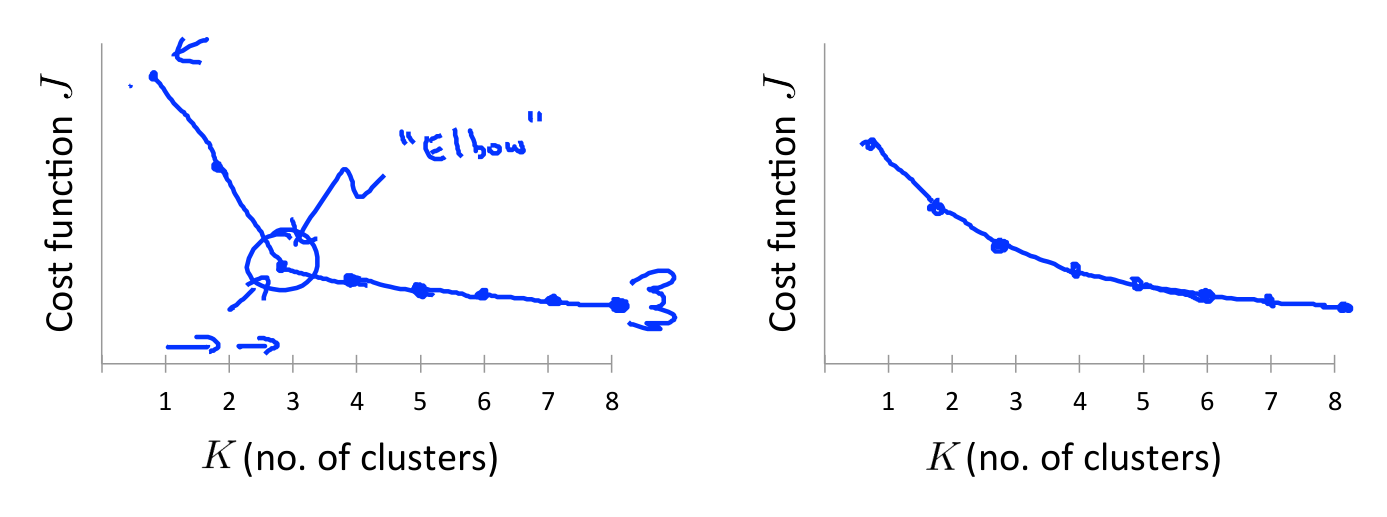
\includegraphics[width=\textwidth]{image/elbow-method.png}
        \caption{Elbow method in apparent cases (left) and non-apparent cases(right)}
        \label{fig:elbow-method}
    \end{figure}

    \par In some cases, there will only be some definitive $K$s to choose from. This is often seen in K-means based on a metric for some downstream purpose. Recall the T-shirt sizing problem, in such cases, we have standard numbers of clusters (3, 5, 7, etc.). One can then iterate through all possible options, and proceed with the one which yields the lowest cost.

    \section{Dimensionality Reduction}

\subsection{Motivation}
    \subsubsection{Data Compression}
    Sometimes there exists redundant data dimensions, e.g. repeated quantities in different units. In general, such dimensions are correlated by some hyperbolic surfaces . In the 2D case, two dimensions $x_1, x_2$ can be compressed into a line that describes the correlation of the two dimensions; thus we need only the information of that "line" and where each pair of ($x_1, x_2$) lies on that line (See Figure \ref{fig:data-compression-2-1}). This can further be generalized into more dimensions, e.g. 3 dimensions lying on a 2D-plane (Figure \ref{fig:data-compression-3-2}). 

    We compress the data by projecting the data points on to the plane of correlation approximation and re-coordinate into $z$. This reduces the data to one-less dimension. 
    \begin{figure}[htpb]
        \centering
        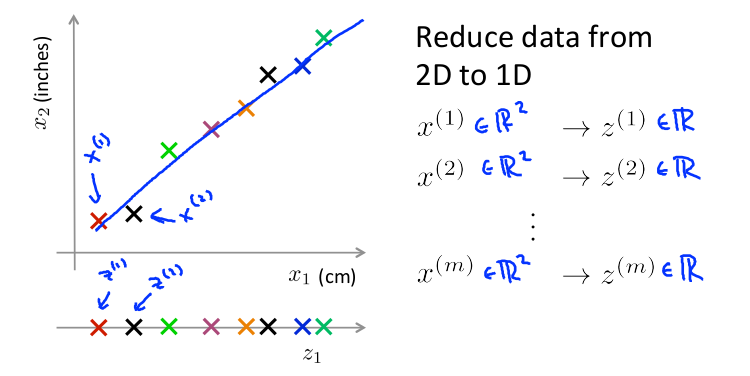
\includegraphics[width=0.8\textwidth]{image/data-compression-2-1.png}
        \caption{Data compression from 2D to 1D}
        \label{fig:data-compression-2-1}
    \end{figure}

    \begin{figure}[htpb]
        \centering
        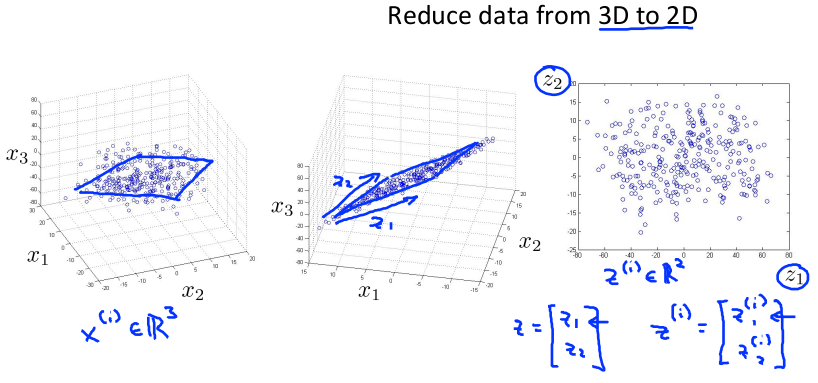
\includegraphics[width=0.8\textwidth]{image/data-compression-3-2.png}
        \caption{Data compression from 3D to 23D}
        \label{fig:data-compression-3-2}
    \end{figure}

    \subsubsection{Data Visualization}
    For visualization purposes, we often wish to group the dimensions into two or three dimensions, of which visualizations are easier perceived by human.

\subsection{Principal Component Analysis}
    \subsubsection{Problem Formulation: n-d to k-d}
    The projection error is the orthogonal distance squared from the data to that projected on the plane.
    To find the plane of correlation approximation, we need to find k vectors: $u^{(1)}, \dots,u^{(k)}$ onto which the data projects, so as to minimize the projection error. We want to project the data onto the linear subspace span by the k vectors. 

    \par For example: from 2D to 1D, we need to find a direction vector ($u^{(1)} \in \mathbb{R}^n$).

    \par Note: \textbf{linear regression is different than PCA.} The former minimizes the squared error $(|y - h(x)|^2)$ (error bar is parallel to the y-axis, not the shortest distance); the latter minimizes the orthogonal distance from the point to the projection. See Figure \ref{fig:linear-regression-PCA} for the comparison.

    \begin{figure}[htpb]
        \centering
        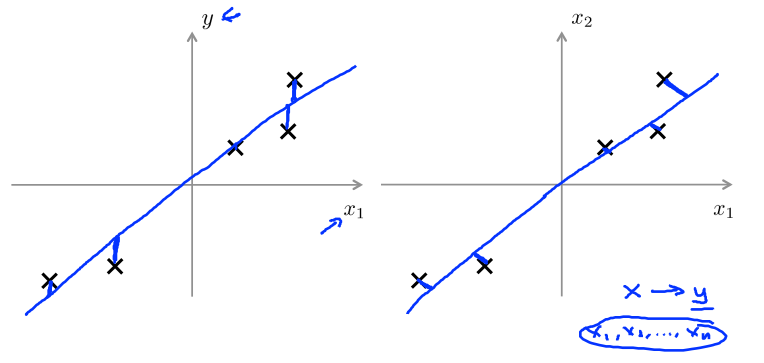
\includegraphics[width=0.8\textwidth]{image/linear-regression-PCA.png}
        \caption{Linear regression vs PCA. Linear regression minimizes the error of y to the prediction. PCA minimizes the error/distance from the original point orthogonal to the projected}
        \label{fig:linear-regression-PCA}
    \end{figure}
\subsection{Principal Component Analysis: Algorithm}
    \subsubsection{Data Preprocessing}
        \begin{itemize}
            \item Training set: $x^{(1)}, x^{(2)}, \dots, x^{(m)}$
            \item Preprocessing (feature scaling and mean normalization):
                \[
                    \mu_j = \frac{1}{m} \sum_{i=1}^{m} x_j^{(i)}
                \] 
                \[
                    x_j^{(i)} \gets \frac{x_j^{(i)} - \mu_j}{s_j}
                \] 
       \end{itemize}

    \subsubsection{Principal Component Analysis}
    Reduce data from n-dimensions to k-dimensions
        \begin{itemize}
            \item Covariance matrix:
                \[
                    \Sigma = \frac{1}{m} \sum_{i=1}^{n} [x^{(i)}][x^{(i)}]^T = \frac{1}{m} X^T X 
                \]

                Recall from Equation \ref{eq:design-matrix}, the design matrix $X$ has each example in a row.

            \item Eigenvectors of $\Sigma$: \verb| [U, S, V] = svd{Sigma}| \\
                  The svd function stands for "single value decomposition". The $U$ matrix is matrix of eigenvectors in columns: 
                  \[
                    U    = \begin{bmatrix}
                    \vertbar    &  \vertbar     &        &     \vertbar \\
                    u^{(1)}     &  u^{(2)}      &  \dots &     u^{(n)}  \\ 
                    \vertbar    &  \vertbar     &        &     \vertbar \\
                           \end{bmatrix}   \in \mathbb{R} ^{n \times n}
                  \] 
              \item Projection: We can take the first k columns from the eigenmatrix U to form $U_{reduce}$:
                  \[
                      U_{reduce}  = \begin{bmatrix}
                        \vertbar    &  \vertbar     &        &     \vertbar \\
                        u^{(1)}     &  u^{(2)}      &  \dots &     u^{(k)}  \\ 
                        \vertbar    &  \vertbar     &        &     \vertbar \\
                                    \end{bmatrix}   \in \mathbb{R} ^{n \times k}
                  \] 
                  Perform the projection:
                  \begin{equation}
                      z^{(i)} = U^T_{reduce} \cdot x^{(i)} \in \mathbb{R}^{k \times 1}
                      \label{eq:pca-projection}
                  \end{equation} 
        \end{itemize}

\subsection{Reconstruction from compressed representation}
    We can guess the original data by inverting \ref{eq:pca-projection}.
    \[
        x \approx x_{approx} = U_{reduce} \cdot z
    \] 

\subsection{Choosing k (num of principal components)}

    \begin{itemize}
        \item Average squared projection error: $\frac{1}{m} \sum_{i=1}^{n} \| x^{(i)} - x_{approx}^{(i)} \| ^2$
        \item Total variation in data: $\frac{1}{m} \sum_{i=1}^{n} \| x^{(i)} \|^2$
        \item Choose k s.t. "99\% variance is retained":
            
            \begin{equation}
                \frac{ \frac{1}{m} \sum_{i=1}^{n} \| x^{(i)} - x_{approx}^{(i)} \| ^2}{\frac{1}{m} \sum_{i=1}^{n} \| x^{(i)} \|^2} \leq  0.01
                \label{eq:pac-metric}
            \end{equation} 
            
        \item Procedure: Try PCA with k=1, compute $U_{reduce}$, check Equation \ref{eq:pac-metric}, $k\gets k+1$.
        \item Implementation note: Equation \ref{eq:pac-metric} can be solved differently using the $S$ matrix. $S \in \mathbb{R} ^{n \times n}$ is a diagonal matrix. For a given k, we can compute Equation \ref{eq:pac-metric} by: 
            \[
                1 - \frac{\sum_{i=1}^{k} S_{ii}}{\sum_{i=1}^{n} S_{ii}}
            \], or alternatively,  
            \[
                \frac{\sum_{i=1}^{k} S_{ii}}{\sum_{i=1}^{n} S_{ii}} \geq 0.99
            \] 

    \end{itemize}
\subsection{Advice for applying PCA}
    \begin{enumerate}
        \item Supervised learning speed-up: define the mapping $x^{(i)} to z^{(i)}$ by running PCA on the \textbf{training set}. This mapping can be later used on cross validation and test sets.
        \item Application of PCA
            \begin{enumerate}
                \item Compression (reduce space), speed up learning algorithm.
                \item Visualization.
                \item \textbf{Bad usage}: prevent overfitting (fewer features, less likely to overfit). However, PCA discards certain information through the projection step. It is better to use regularization ($\lambda$)
            \end{enumerate}
        \item Design ML system without PCA first, if that doesn't work, then try PCA.
    \end{enumerate}

    \section{Anomaly Detection}
    \subsection{Motivation: Density Estimation}
        Generate a function \emph{p(x)}, such that $p(x) < \epsilon$ suggest anomaly. 
        The crux is to flag unusual behaviour, for example: 
        \begin{itemize}
            \item Fraud detection
            \item Manufacturing 
            \item Computer load in data center
        \end{itemize}

        \subsubsection{Guassian distribution}
            \begin{equation}
                x \sim \mathcal{N}(\mu, \sigma^2)
                \label{eq:guassian}
            \end{equation}

            \begin{itemize}
                \item $\mu$: mean
                \item $\sigma^2$: variance
            \end{itemize}

    \subsection{Algorithm}
        \begin{enumerate}
            \item Choose features $x_i$ that are indicative of anomalous examples. 
            \item Fit parameters 
                \begin{equation}
                \boldsymbol{\mu} = \begin{bmatrix}
                                            \mu_1       \\
                                            \vdots      \\
                                            \mu_i       \\
                                            \vdots      \\
                                            \mu_n       
                                        \end{bmatrix} = \frac{1}{m} \sum_{i=1}^{m} x_j^{(i)}
                    \label{eq:anomaly-mu}
                \end{equation} 
                                        and 
                \begin{equation}
                \boldsymbol{\sigma^2} = \begin{bmatrix}
                    \sigma^2_1       \\
                    \vdots      \\
                    \sigma^2_i       \\
                    \vdots      \\
                    \sigma^2_n       
                \end{bmatrix} = \frac{1}{m} \sum_{i=1}^{m} (x^{(i)} - \mu)^2
                    \label{eq:anomaly-sigma-squared}
                \end{equation}
        \item Given new example $x$, compute $p(x)$: 
                \begin{equation}
                    p(x) = \prod_{j=1}^{n} p(x_j;\mu_j, \sigma^2_j) = \prod_{j=1}^{n} \frac{1}{\sqrt{2 \pi} \sigma_j} exp(\frac{-(x_j - \mu_j)^2}{2 \mu_j ^2})
                    \label{eq:anomaly-p}
                \end{equation}

            Anomaly if $p(x) < \epsilon$

        \end{enumerate}
    \subsection{Developing and Evaluating an Anomaly Detection System}
        Dividing labelled data:
        \begin{itemize}
            \item Training set: 60\%.
            \item Cross validation set: 20\%
            \item Test set: 20\%.
        \end{itemize}
    
    \subsection{Anomaly Detection vs Supervised Learning}
    Refer to Table \ref{tab:anomaly_detection_vs_supervised_learning}. 

    \begin{table}[htpb]
            \centering
            \begin{tabular}{|p{0.5\linewidth}|p{0.5\linewidth}|}
                \hline
                Anomaly detection & Supervised learning \\
                \hline
                Small number of positive examples [y=1] (0-20) and large number of negative examples [y=0] & Large number of positive and negative examples \\
                \hline 
                Many different types of anomalies. Hard to learn anomalies from positive examples.  & Enough positive examples to learn positivity. \\
                \hline 
                Future anomalies may look nothing like previous anomalies & Future positive examples similar to training set.\\
                \hline
            \end{tabular}
            \caption{Anomaly detection vs Supervised learning}
            \label{tab:anomaly_detection_vs_supervised_learning}
        \end{table}
    
    \section{Choosing what features to use}
        \begin{itemize}
            \item \textbf{Goal}: Want $p(x)$ large for normal examples x; $p(x)$ small for anomalous examples x. 
            \item Ideally require Guassian features. 
            \item If not Guassian, require preprocessing, e.g. log(), $\sqrt{x}$, etc. 
            \item Most common problem: $p(x)$ is comparable for both normal and anomalous examples $\rightarrow$ come up with new features (e.g. ratios of current fetatures. )
        \end{itemize}
            
    \subsection{Multivariate Guassian Distribution}
        
    $x \in \mathbb{R}^n$. Model $p(x)$ with all dimensions in tandem. Parameters: $\boldsymbol{\mu} \in \mathbb{R}^n$, $\Sigma \in \mathbb{R}^{n \times n}$ (covariance matrix).
        
        \subsubsection{Anomaly detection using multivariate Guassian distribution}
        \begin{equation}
            p(x; \mu, \Sigma) = \frac{1}{(2\pi)^{n/2} |\Sigma|^{1/2}} exp (- \frac{1}{2} (x -\mu)^T \Sigma ^{-1} (x-\mu))        
            \label{eq:multivariate_anomaly_p}
        \end{equation}
        where 
            \begin{equation}
                \mu = \frac{1}{m} \sum_{i=1}^{m} x^{(i)}
                \label{eq:anomaly-mu-2}
            \end{equation}

            \begin{equation}
                \Sigma = \frac{1}{m} \sum_{i=1}^{m} (x^{(i)}-\mu) (x^{(i)}-\mu)^T
                \label{eq:}
            \end{equation}


        \subsubsection{Original model vs Multivariate Guassian}
            \begin{table}[htpb]
                \centering
                \begin{tabular}{|p{0.5\linewidth}|p{0.5\linewidth}|}
                    \hline
                    Original model & Multivariate Guassian \\
                    \hline
                    $\prod_{j=1}^{n} p(x_j;\mu_j, \sigma^2_j)$ (Eq. \ref{eq:anomaly-p} )& Eq. \ref{eq:multivariate_anomaly_p} \\
                    \hline
                    Manually combine features to capture anomalies & Automatically captures correlations between features. \\
                    \hline
                    Computationally cheaper and scales well & Computationally expensive (matrix) \\
                    \hline 
                    Works on small training set size (m) & Must have training set size (m) $>$ features size (n), i/e/ m $geq$ 10n for $\Sigma$ to be invertible.\\
                    \hline
                    
                \end{tabular}
                \caption{Anomaly detection: original model vs multivariate Guassian}
                \label{tab:anomaly-origin-multivariate}
            \end{table}

    \section{Recommender Systems}
    \subsection{Problem formulation}
        \begin{enumerate}
            \item X = $\left\lbrack 
                \begin{array}{c}
                    -{\;\left(x^{\left(1\right)} \right)}^T -\\
                    -{\;\left(x^{\left(2\right)} \right)}^T -\\
                    \vdots \\
                    -{\;\left(x^{\left(n_m \right)} \right)}^T -
                \end{array}
                \right\rbrack$  For each movie $i$ ($i = 1 \dots n_m$), form a feature vector $x^{(i)}$ to characterize the movie. 
            \item $\Theta$ = $\left\lbrack 
                \begin{array}{c}
                    -{\;\left(\theta^{\left(1\right)} \right)}^T -\\
                    -{\;\left(\theta^{\left(2\right)} \right)}^T -\\
                    \vdots \\
                    -{\;\left(\theta^{\left(n_u \right)} \right)}^T -
                \end{array}
                \right\rbrack$ For each use $j$ ($j = 1 \dots n_u$), there is a parameter vector $\theta^{(j)}$ that characterizes the user's interest, such that $(\theta^{(j)})^T x^{(i)}$ is a prediction of user $j$'s rating on movie $i$. 
            \item $Y$ = \{ $y(i,j)$ \}, where $y(i,j)$ is the actual ratings of use $j$ on movie $i$.
            \item $R$ = \{ $r(i,j)$ \}, where $r(i,j)$ is the "valid" bit for $y(i,j)$, i.e. if user $i$ gave a rating on movie $i$.
        \end{enumerate}
    \subsection{Collaborative filtering}
    The cost function for collaborative filtering with regularization is: 
        \begin{equation}
            J(X, \Theta)=
\frac{1}{2}\sum_{(i,j):r(i,j)=1}\left((\theta^{(j)})^Tx^{(i)}-y^{(i,j)}\right)^2+\left(\frac{\lambda}{2}\sum_{j=1}^{n_u}{\sum_{k=1}^{n}{(\theta_k^{(j)})^2}}\right)+\left(\frac{\lambda}{2}\sum_{i=1}^{n_m}{\sum_{k=1}^{n}{(x_k^{(i)})^2}}\right)
            \label{eq:collab-filter-reg}
        \end{equation}

    One can then apply gradient descent: 

    \begin{equation}
        \theta^{(j)}_k := \theta^{(j)}_k - \alpha   \sum_{i:r(i,j) = 1}^{} \frac{\partial }{\partial \theta_k^{(j)}} J(X, \Theta)
        \label{eq:collab-filter-reg-grad-desc-theta}
    \end{equation}
    \begin{equation}
        x^{(i)}_k := x^{(i)}_k - \alpha   \sum_{i:r(i,j) = 1}^{} \frac{\partial }{\partial x_k^{(j)}} J(X, \Theta) 
        \label{eq:collab-filter-reg-grad-desc-x}
    \end{equation}

    where
    \begin{equation}
\frac{\partial J}{\partial x_k^{(i)}} = \sum_{j:r(i,j)=1}\left((\theta^{(j)})^T 
x^{(i)} -y^{(i,j)}\right)\theta_k^{(j)}+\lambda x_k^{(i)}
        \label{eq:collab-filter-grad-Jx}
    \end{equation}
    \begin{equation}
\frac{\partial J}{\partial \theta_k^{(j)}} = \sum_{i:r(i,j)=1}\left((\theta^{(j)})^T x^{(i)} -y^{(i,j)}\right) x_k^{(i)}+\lambda\theta_k^{(j)}
        \label{eq:collab-filter-grad-Jtheta}
    \end{equation}


    The collaborative filtering algorithm is:
    \begin{enumerate}
        \item Initialize $x^{(i)}, \theta^{(j)}$ to small random values. 
        \item Minimize $J(X, \Theta)$ using gradient descent.
        \item Predict user $i$ rating on movie $j$ via $(\theta^{(j)})^T x^{(i)}$
    \end{enumerate}

    \section{Gradient Descent with Large Datasets}
\subsection{Stochastic gradient descent}
\begin{itemize}
    \item \textbf{Batch gradient decent}:  In each iteration, sum cost of all \emph{m} examples, then taking one step of minimization (improving parameters). Might be expensive as number (of training examples) scales up.
    \item \textbf{Stochastic gradient descent}: take single cost of a training example, start improving the parameters towards global minimum. The algorithm may not converge immediately in a direct path; the route taken might be conservative and biased towards each individual sample. Might not converge to a single minimum; algorithm might end up wandering near the minimum-- this is a "good enough" hypothesis in most cases. Usually 1-10 iterations.
    \item \textbf{Mini-batch gradient descent}: use \emph{b} examples in each iteration (rather than all m). Step in size of \emph{b}. Also faster than Batch gradient descent. Outperforms Stochastic gradient descent if good vectorization can be performed (achieve parallelism). Downside: extra variable b.
\end{itemize}
\subsection{Stochastic gradient descent convergence and tuning}
\par Recall for Batch gradient descent, we had to plot $J_{train} (\theta)$ as a function of number of iterations of gradient descent. 

\par For Stochastic gradient descent, during learning, compute $cost(\theta, (x^{(i)}, y^{(i)}))$ before updating $\theta$ using $(x^{(i)}, y^{(i)})$. For every 1000 iterations, plot averaged over last 1000 examples. This gives a running estimate of how well minimization performs. IF we see that the running estimate increases over time, we can try to use a smaller learning rate $\alpha$; each iteration of the stochastic gradient descent will take a smaller step, thereby increasing the likelihood of convergence. 





\subsection{Advanced topic: online learning}
\begin{itemize}
    \item Take one example, improve parameters based on the single example (this is essentially stochastic gradient descent). Discard example. 
    \item Useful when website gets a stream of data from different users. 
    \item Can adapt to varying user preference.
    \item Search query keywords (Predicted CTR Click-through-rate): $p(y=1 | x;\theta)$.
\end{itemize}
\subsection{Advanced topic: map reduce and data parallelism}
\begin{itemize}
    \item Split examples into batches for different machines. 
    \item Each machine will compute semi-total cost according to the batch it was assigned. 
    \item Combine calculated cost to perform gradient descent and get a single $\theta$.
    \item Net result is equivalent to original 
    \item Applicable to multi-core machines: no network latency.
\end{itemize}

\begin{figure}[htpb]
    \centering
    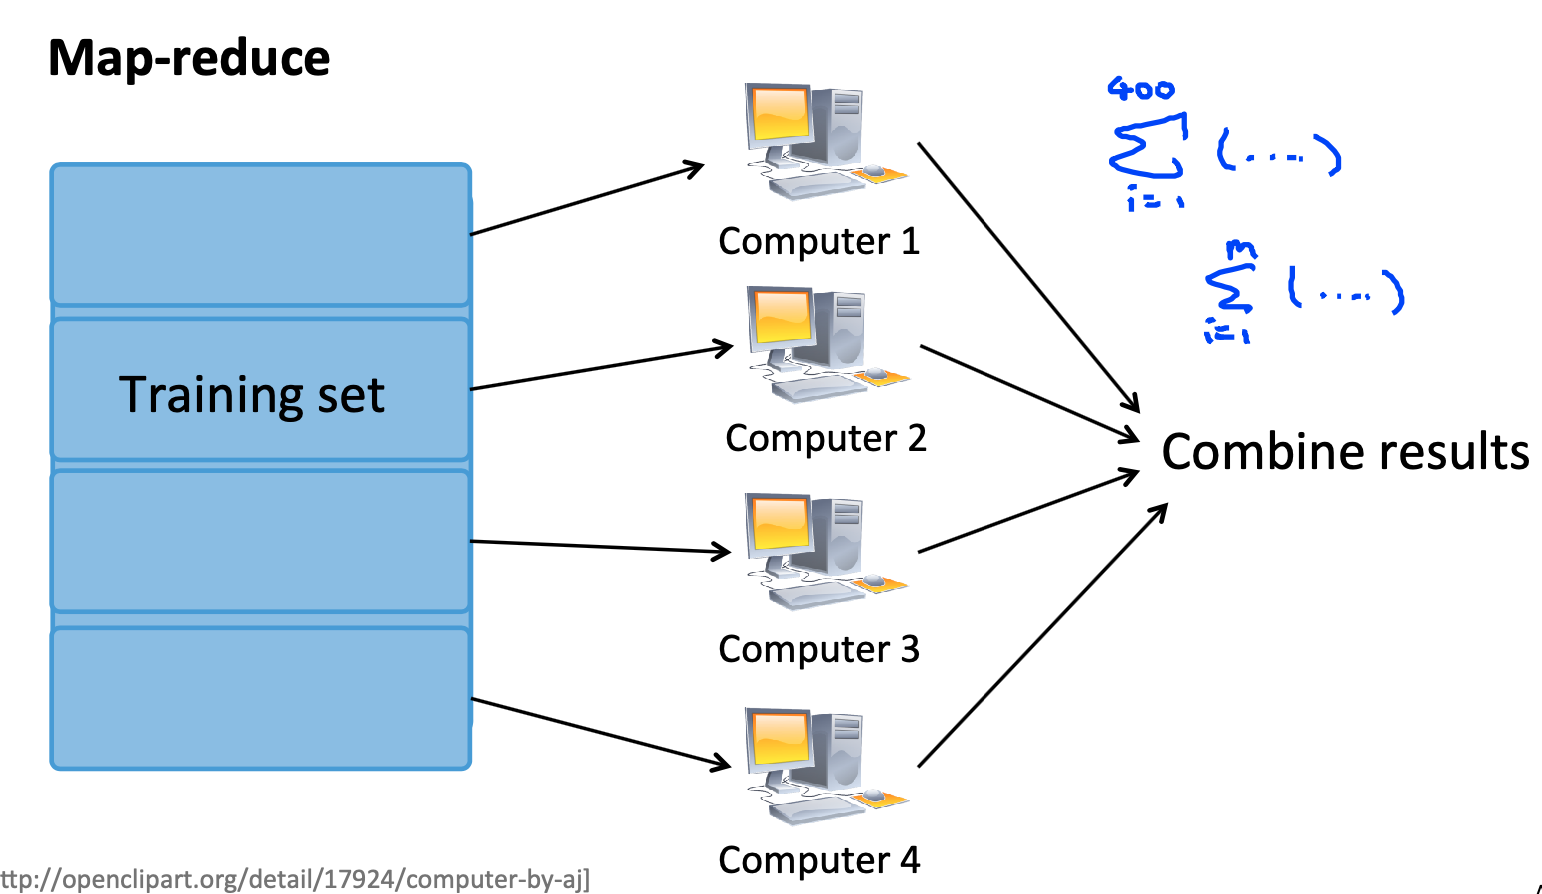
\includegraphics[width=0.8\textwidth]{image/map-reduce.png}
    \caption{Map reduce}
    \label{fig:map-reduce}
\end{figure}

\subsection{Stochastic gradient descent applications}
\par Many learning algorithms can be expressed as computing sums of functions over the training set; map-reduce is good candidate for such algorithms, where the bottleneck stems from summing over the training set. Because of network latency and other overhead, if we run map-reduce on N computers, we might get less than an N-fold speedup.
\begin{itemize}
    \item Batch gradient descent: split dataset into N smaller batches, compute the gradient for each smaller batch on each machine, then average the gradients on a central computer for the gradient update. This works for regressions and neural network training
    \item Stochastic gradient descent: \textbf{Not applicable}. Since stochastic gradient descent processes one example at a time and performs update after each example, it cannot be easily parallelized.
\end{itemize}




\end{document}


